% Terms and Definitions
\chapter{Web Performance} % korrigiert
\label{chapter:web_performance}

%TODO roter faden: What is web performance in web analytics context ?

% [Last chapter]

In the last chapter, we saw how important performance is in e-commerce and how web analytics help measure many aspects of e-commerce websites.
This provides the context for the following chapter.

% [This chapter]

This chapter is about web performance.
Web performance is also about analysing the website, but not about business-related issues such as the type of users, how they interact with the website, or whether they lead to conversions.
Web performance is about the website itself, specifically how fast it is and how users perceive performance.

The introduction section \ref{section:web_performance_introduction} gives an overview of some general ideas and aspects of web performance.
Some of them will be discussed in more detail.
To understand web performance, one must know how websites are loaded into the browser and presented to the user.
Section \ref{section:website_loading_process} explains this process, focusing on the steps within the network and the front end.
What techniques exist for measuring and evaluating the performance of a website are discussed in section \ref{section:measurement_methods}.
Finally, section \ref{section:web_performance_metrics} discusses metrics that reflect and capture the performance of a website.


% [Relevance of this chapter for research question] ??


% [Next chapter]

Before describing the approach and practical work done to address the research question in chapter \ref{chapter:approach}, the next chapter \ref{chapter:related_work} discusses some other research in this area.



% ---------------------------------------------------------------------------------------------------
% ---------------------------------------------------------------------------------------------------

\section{Introduction} % korrigiert
\label{section:web_performance_introduction}

% [Introduction]

As described in section \ref{chapter:user_satisfaction}, web performance plays a non-negligible role in user satisfaction and business success.
The studies cited in the relevant section show that increasing website performance also increases sales, or as Google puts it, "Performance plays a major role in the success of any online venture."\footnote{\url{https://web.dev/why-speed-matters/} [03.06.2021]}

A good overview of web performance topics and goals is provided by the MDN Web Docs\footnote{\url{https://developer.mozilla.org/en-US/docs/Learn/Performance/What_is_web_performance} [03.06.2021]}, which serve as an outline for this chapter and are briefly described below.


\paragraph{Reducing load time} % korrigiert

To understand how load times occur, the technical aspect of how websites are loaded and presented to the user by the browser must be understood.
This subject is addressed in section \ref{section:website_loading_process}.

Concrete optimization steps and techniques to reduce loading times are not the subject of this work.


\paragraph{Usability and interactivity} % korrigiert

There are several metrics that attempt to reflect areas of performance such as load time, smoothness, and interactivity, and there are specific metrics to distinguish between technical and user-perceived performance.
Web performance metrics are discussed in section \ref{section:web_performance_metrics}.


\paragraph{Performance perception} % korrigiert

Perceptions of performance are generally subjective.
As seen earlier in section \ref{chapter:user_satisfaction}, there are some quantifiable time intervals that correlate with human psychology regarding received performance.
Table \ref{table:perception} provides "unofficial rules of thumb" for delay thresholds \cite{2013Grigorik}.

\begin{table}[h]
	\small
	\centering
	\begin{tabular}{| l | l | }
	\hline
	Delay \cellcolor{lightgrey} & User Perception \cellcolor{lightgrey} \\
	\hline
	0-100 ms & Instant \\
	100-300 ms & Small perceptible delay \\
	300-1000 ms & Machine is working \\
	> 1 s & Likely mental context switch \\
	> 10 s & Task is abandoned \\
	\hline
	\end{tabular}
	\medskip
	\caption{Rule of thumbs for delay}
	\label{table:perception}
\end{table}

Interpreting the numbers from the table, one can make the statement that it is desirable to keep load times below one second.
Thresholds for certain performance metrics and the psychological rationale for setting them are briefly discussed in section \ref{subsubsection:core_web_vitals}.


% TODO add this?
% https://developer.mozilla.org/en-US/docs/Learn/Performance/why_web_performance
% financial aspect of downloading data and big websites


\paragraph{Performance measurements} % korrigiert

Measuring the performance of a website is an important and non-trivial task.
Two main methods for measuring the performance of a website exist:
\textit{Synthetic Monitoring} is discussed in section \ref{subsection:synthetic_monitoring},
\textit{Real User Monitoring} (RUM) is covered in section \ref{subsection:RUM}.

% ---------------------------------------------------------------------------------------------------

\section{The Website Loading Process} % korrigiert
\label{section:website_loading_process}

% [Introduction]

To understand web performance metrics and the methods used to measure them, it is critical to have a basic understanding of the technical aspect of loading a web page into the browser. 
In general, this process involves establishing a connection between a client and a server, and the browser's task of converting the data received from the server into a readable, ready-to-use website.

% [3 Entities: FE, BE, Network]

It is helpful to divide the components of the website loading process into three units: The front-end, the back-end, and the network. % cite 2016 Witt ??
The front-end takes care of everything the user sees on the screen, such as rendering the UI, and consists of a client (browser) that requests data from the back-end.
The back-end, usually a web server, processes the client's requests and sends the response back to the front-end.
The data is transmitted over the network, which connects the front and back ends and consists of network components such as cables, routers, switches, network protocols, and so on.

Figure \ref{figure:timing_overview} shows the three entities and their tasks during the website loading process.
What happens in the network phase is described in section \ref{subsection:network_process}.
The front-end's task of receiving data and transforming it into a website is covered in section \ref{subsection:crp}.
How the back-end processes requests and creates responses is not part of this work.

\begin{figure}[h!]
\begin{center}
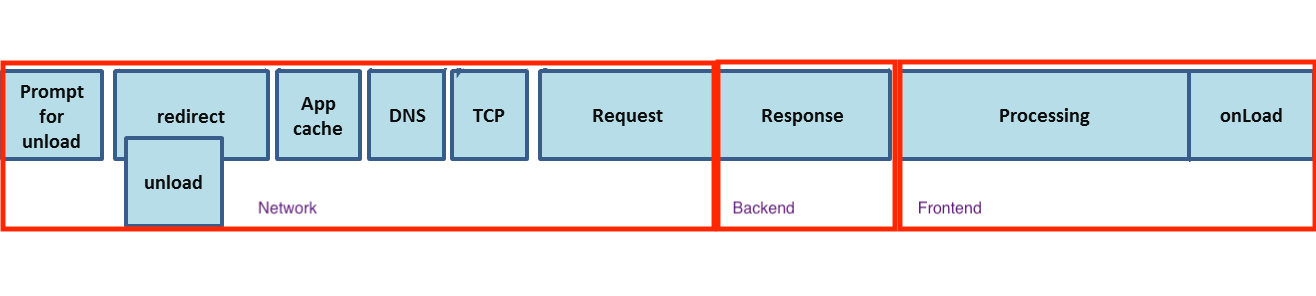
\includegraphics[width=0.8\textwidth]{timing_overview_blanco2.png}
\caption{Timing Overview}
\label{figure:timing_overview}
\end{center}
\end{figure}
%TODO change image: make it clean



% --------------------------------------------------------------------------------------------
% --------------------------------------------------------------------------------------------


\subsection{The Website Loading Process in the Network} % korrigiert
\label{subsection:network_process}

The network connects the front-end to the back-end.
When a client requests resources from a server, data must be transferred over the network.

Latency and bandwidth are two important factors in network performance.
How they affect performance is discussed in section \ref{subsubsection:latency_bandwidth}.
The procedure and other mechanisms for establishing a reliable and secure connection between the front-end and the back-end are described in section \ref{subsubsection:network_navigation_steps}.
Web performance metrics measure, among other things, how long certain steps take during connection establishment, as described in section \ref{subsection:navigation_timing_metrics}.


% --------------------------------------------------------------------------------------------


\subsubsection{Latency and Bandwidth} % korrigiert
\label{subsubsection:latency_bandwidth}

There are two important factors when discussing network performance: latency and bandwidth.
As will be examined below, latency is the bottleneck of network performance, not bandwidth.

% [Bandwidth]

Bandwidth is the "maximum throughput of a logical or physical communication path" \cite{2013Grigorik}.
In other words, bandwidth describes the amount of data that can be sent in parallel from one node in a network to another. 
Physical communication paths are usually cables such as metal wires or fiber optic cables, with fiber optic cables having less signal loss and lower lifetime maintenance costs.
Using methods such as wavelength division multiplexing (WDM), it is possible to transmit up to 70 Tbit/s over a fiber optic link.
This high technology is only used in the backbone infrastructure, e.g. for the connection between Europe and America.
For the end user, the bandwidth is much lower, and the average was only 5.1 Mbit/s at the end of 2015.
High bandwidth is useful for bulk or large-scale data transfers like streaming video or audio.
But for loading a website or any other browser activity that depends on many requests fetching data from many different locations around the globe, the performance bottleneck is latency \cite{2013Grigorik}.

% [Latency]

Latency is "the time from the source sending a packet to the destination receiving it" \cite{2013Grigorik}.
Latency is measured in seconds and can be the time it takes to travel a single distance or, more commonly, how long it takes the transmitted data packet to round-trip time (RTT) from source to destination and back.
In other words, latency "describes the amount of delay on a network or Internet connection" \cite{2021MDNLatency}.
For the very first request when establishing a connection, the latency is longer due to protocols such as DNS lookups, TCP and TLS handshakes \cite{2021MDNLatency}.
These are discussed in section \ref{subsubsection:network_navigation_steps}.

% [Experiment]

To get an idea of how the two aspects of bandwidth and latency affect web performance, Mike Belshe conducted a study \cite{2010Belshe}:
There are two configurations. One has fixed latency and variable bandwidth, and the other is configured the other way around.
He then compared the performance of the two configurations using the Page Load Time metric (figure \ref{figure:latency}).


\begin{figure}[h!]
\begin{center}
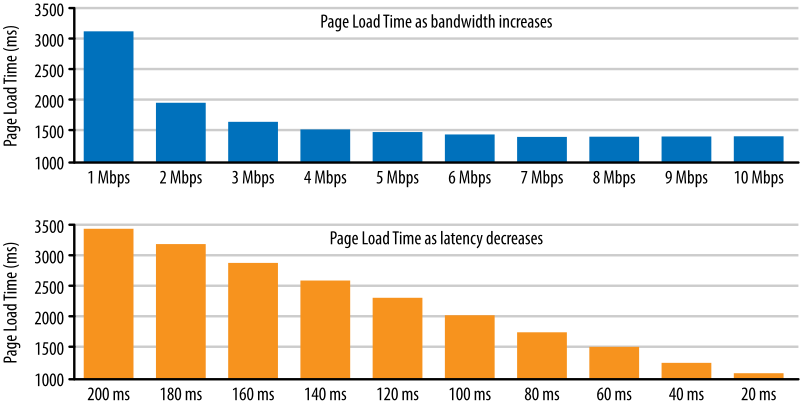
\includegraphics[width=0.8\textwidth]{latency.png}
% \caption{Latency vs Bandwidth, taken from \cite{2013Grigorik}}
\caption[Latency vs Bandwidth]{Latency vs Bandwidth, taken from \cite{2013Grigorik}}
\label{figure:latency}
\end{center}
\end{figure}


We see that the influence of the bandwidth is trivial: if the available bandwidth is doubled, e.g. from 5 to 10 Mbit/s, there is no change in the loading time.
For latency, on the other hand, the picture is different: If the latency can be reduced by half, e.g. from 120 ms to 60 ms, the page load time also drops by half.
Or as Belshe puts it, "[reducing] cross-atlantic RTTs from 150ms to 100ms [...] would have a larger effect on the speed of the internet than increasing a user's bandwidth from 3.9Mbps to 10Mbps or even 1Gbps" \cite{2010Belshe}.

These observations can be explained by the many short, small connections and requests made while browsing websites and the contrary basic structure of the communication protocols, which are "optimized for long-lived connections and bulk data transfers" \cite{2013Grigorik}. % add ch 10 ?
But simply reducing latency is not easy: the speed of data transmission is already 2/3 the speed of light, but the physical conditions are the limiting factor, e.g. there is a minimum distance between London and New York that cannot be "optimized" further \cite{2013Grigorik}. % add Ch 1 ?

% add more here? Why is this here?


% [Mobile]

Another aspect of latency is that latency is even higher for wireless connections and thus for mobile devices, "making network optimization a critical priority for the mobile web" \cite{2013Grigorik}. % add Ch 1
Latency is high for mobile users due to mobile network infrastructure (see also "Why are mobile latencies so high?" in \cite{2013Grigorik}).


% [Transition]

Although latency is an important factor, what happens on the front end is still important.
At the same time, this thesis focuses on metrics to measure performance on the front end.
Before going into what happens in the browser once the website data arrives, I will briefly describe the preceding steps of establishing a connection between the browser (client) and the server, which can still be considered part of the network.


% add this ?
% Use other techniques such as CDNs, caching, pre-fetching, etc % 2013 Grigorik
% CDN: Help against this issue. Put stuff close to client % 2013 Grigorik
% Some direct implications for performance measurement ?
% Understanding Latency https://developer.mozilla.org/en-US/docs/Web/Performance/Understanding_latency
% Network throttling: Emulate download speed, upload speed, and minimum latency


% --------------------------------------------------------------------------------------------

\subsubsection{Network Navigation Steps} % korrigiert
\label{subsubsection:network_navigation_steps}

When the user enters a URL into the browser, a series of steps are taken to render and present the website to the user.
These steps consist of DNS lookup, TCP and TLS negotiation, and the HTTP request, among others.
These steps are necessary to establish a secure and reliable connection between the browser (client) and the server, and are described below.

% add this ?
% "To start, it is important to recognize that every HTTP request is composed of a number of separate stages [...]: DNS resolution, TCP connection handshake, TLS negotiation (if required), dispatch of the HTTP request, followed by content download." % cite Grigorik 2013
% Understanding Latency https://developer.mozilla.org/en-US/docs/Web/Performance/Understanding_latency
%Network Timings:
%- Blocked: When a request is in queue
%- Blocking happens when there are too many simultaneous connections to single server over HTTP


% ----------------------------------


\paragraph{DNS Lookup} % korrigiert

If the requested resource cannot be loaded from the browser's cache, the first step in establishing a connection is a DNS (Domain Name System) lookup (or DNS resolution).

This step is about translating the URL into an IP address.
It must be performed for each unknown URL, for example, if linked images on a website come from different servers, a DNS lookup must be performed for each individual URL.
The URL to IP mapping can be cached by the browser, which makes repeated calls faster \cite{2021MDNHowBrowsersWork}.

DNS lookups take between 20 and 120 milliseconds on average \cite{2018KeyCDN}.

% Metric?
% Can be considered a performance metric, see section X.


% ----------------------------------


\paragraph{TCP Handshake} % korrigiert

The goal of TCP (Transmission Control Protocol) is to establish a reliable connection in an unreliable network.
TCP  "guarantees that all bytes sent will be identical with bytes received and that they will arrive in the same order to the client" \cite{2013Grigorik}.
The TCP 3-way handshake is a technique for establishing a reliable connection.
In terms of performance, the handshake adds two more roundtrips, which, as we have seen, is bad for performance because of latency.

There are many algorithms and techniques for optimal data transmission and avoiding congestion, e.g. Slow-Start.
Slow-Start is an algorithm that determines the maximum usable bandwidth by gradually increasing the amount of data sent.
Slow-Start prevents the full capacity of the network from being used from the start, which in turn leads to more round trips and latency \cite{2013Grigorik}.
For a detailed discussion of TCP, see "Building Blocks of TCP" in \cite{2013Grigorik}.

% once i know which metric add it here ?
%A performance metric reflecting the time spent for establishing a TCP connection is X, see section X.


% ----------------------------------


\paragraph{TLS Negotiation} % korrigiert

TLS (Transport Layer Security) is another protocol whose goal is to establish a secure connection in the sense of data encryption.
Data that is transmitted over the network must be encrypted so that outsiders cannot read or manipulate the data.
For encryption, a cipher must be defined that is exchanged between client and server during TLS negotiation \cite{2021MDNHowBrowsersWork}.

From a performance perspective, TLS in turn means more roundtrips, which has a negative impact on performance.
For a detailed discussion of TLS, see "Transport Layer Security (TLS)" in \cite{2013Grigorik}.

% once i know which metric add it here?
% A performance metric reflecting the time spent for a TLS negotiating is blabla in section X.


% ----------------------------------


\paragraph{HTTP Request and Response} % korrigiert

Now that a secure connection has been established, the client fetches the first resources via HTTP GET request.
In most cases, the server responds by returning the index.html file, which can then be used by the browser to build the website \cite{2021MDNHowBrowsersWork}.

% add this ? Then i would probably mention all metrics here already...
% The time taken by this first response, which contains the first byte to build the site, is reflected in the metric TTFB, which is explained in section X.

% [Connection vs Request]

Normally, many more resources are requested from the browser to complete the construction of the website.
Currently, the average is about 70 requests per website \cite{2021HTTPArchiveStateOfTheWeb}.

A request is not the same as a connection:
Once the connection is established using the methods described above, such as DNS lookup, TCP, and TLS handshakes, multiple requests can be transmitted over the same connection.
Typically, the number of requests is much higher than the number of connections to load a website because the browser maintains connections to keep them open for multiple requests.
The average number of connections for a website today is about 13 \cite{2021HTTPArchiveStateOfTheWeb}.
Modern browsers like Chrome allow up to six connections open in parallel \cite{2014Hogan}. \\


% [Transition to CRP]

At this point, the browser has received the first data about the website and it can start rendering the page.
Exactly how this happens is explained in the next section.


% --------------------------------------------------------------------------------------------
% --------------------------------------------------------------------------------------------


\subsection{The Website Loading Process in the Frontend: Critical Rendering Path} % korrigiert
\label{subsection:crp}

This section explains what happens after the first bytes of the website arrive in the browser.
The following processes are usually subsumed under the term \textit{Critical Rendering Path} (CRP).
The CRP is the final part of the navigation process, as shown in figure \ref{figure:timing_overview}.


% [Critical]

The CRP is the minimum number of steps the browser must take from receiving the first HTML byte to rendering pixels on the screen for the first time.
Rendering is "critical" because it is the very first rendering, the first visible content the user sees on the screen.
The resources needed to render the page for the first time are considered critical.
Without the critical resources, the browser cannot display the content on the screen.
An example of a critical resource is the first HTML file that the browser receives, because without it, nothing can be seen on the screen.
Non-critical resources, on the other hand, do not prevent the browser from displaying the first content on the screen \cite{2018Johnson}.


% [CRP Steps]

There are a number of steps that the browser goes through to render the page.
The basic idea is to convert HTML, CSS, and JS into actual pixels on the screen.

Figure \ref{img:crp} illustrates the flow of the CRP:
Once the HTML code is received, the browser starts parsing the HTML code and translates it into the DOM.
The content of the CSS files is parsed into the CSSOM.
JavaScript must be retrieved and executed.
Once the DOM and CSSOM are available, the render tree is created.
When the render tree is available, the layout is created.
Finally, the pixels can be output to the screen \cite{2021MDNCRP}.

The individual steps are described in more detail below.


\begin{figure}[h!]
\begin{center}
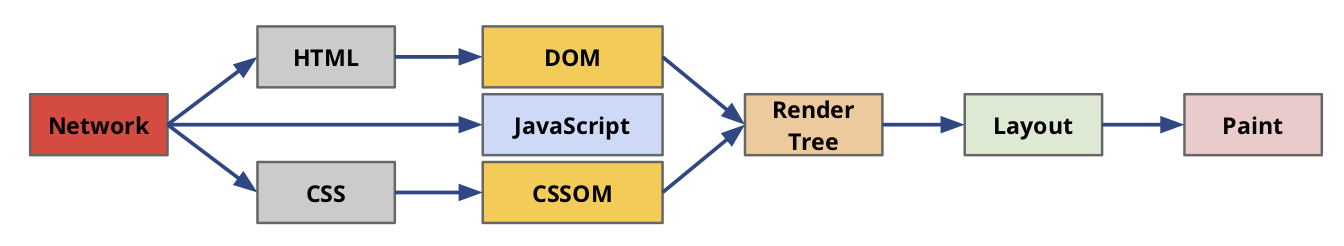
\includegraphics[width=0.7\textwidth]{crp.png}
\caption{Critical Rendering Path}
\label{img:crp}
\end{center}
\end{figure}



% [Single Thread]
% do i need this ?
% How Browsers Work https://developer.mozilla.org/en-US/docs/Web/Performance/How_browsers_work
%- This is somewhat the bottleneck or the technical state of the browser
%- Browser is single threaded
%- Still: Enable smooth interaction: scrolling, responsive to touch, etc.
%- Render time is key
%- Goal: Main thread can complete all the work and still is available to handle user interaction
%-> Improvement: Understand single thread concept of browser and minimize main threads responsibilities
%-> Should lead to: rendering is fast and smooth and responses to interactions are immediate



\paragraph{DOM Construction from HTML} % korrigiert

% [Introduction, Standard]

As soon as the browser receives the first bytes of the HTML file, it begins to decompose it into the \textit{Document Object Model} (DOM).
Building the DOM is the first step the browser takes when it receives data.
The DOM is a tree structure and an internal representation of the HTML for the browser \cite{2021MDNHowBrowsersWork}.

The general parsing process consists of translating bytes into characters, into tokens, into nodes, and finally into the object model \cite{2019GrigorikDOM}.
The specification of the DOM is maintained by the WHATWG living standard (for standards, see section \ref{subsubsection:web_standards}).

% The Parsing of the HTML into the DOM is defined in the HTML standard % footnote https://html.spec.whatwg.org/multipage/parsing.html#parsing


% [Render Blocking]

The DOM tree contains information about the content of the document, but not about its style.
The styling is defined in the CSS (see next section).
Once HTML and CSS have been transferred and processed by the browser, the \textit{Render Tree} can be created to reflect the actual information and its styling that the browser can display.
In this context, it is possible to categorize resources into render-blocking and non-render-blocking:
A render-blocking resource is a resource that prevents the browser from rendering the content on the screen.
HTML and CSS are render-blocking resources because the parsing process of these files prevents the browser from rendering the page on the screen \cite{2019GrigorikCSS}.

% CSS parsing and render tree construction will be discussed below.

% [Incrementally]

As soon as the first data packets of HTML arrive in the browser, the parsing process begins \cite{2021MDNHowBrowsersWork}.
The DOM is created incrementally, which means that the browser can begin processing the HTML before all of the content is transmitted over the network.

% [Resources]

Usually, external resources are linked in the HTML code that are necessary for the completeness of the website, such as CSS or JavaScript.
When parsing the HTML step by step, a reference to such an external resource will appear at some point.
How the external resources CSS and JavaScript are handled by the browser is explained below.


% add this?
% How Browsers Work https://developer.mozilla.org/en-US/docs/Web/Performance/How_browsers_work
%- DOM is also exposed, and can be manipulated through various APIs in JavaScript 
%Optimisation: Preload scanner:
%- This process occupies main thread while browser is building DOM Tree
%- parse through the content available and request high priority resources like CSS, JavaScript, and web fonts.
%- will retrieve resources in the background so that by the time the main HTML parser reaches requested assets, they may possibly already be in flight, or have been downloaded


% ------------------------------------------------------------


\paragraph{CSSOM Construction from CSS} % korrigiert

% [Introduction]

The CSS resource contains all the information about the styling of the page.
As with HTML, CSS is converted from bytes to characters, tokens, nodes, and finally to the \textit{CSS Object Model} (CSSOM) \cite{2019GrigorikDOM}.
CSSOM construction is usually very fast and is standardized by the W3C \cite{2021MDNHowBrowsersWork}.

% The DOM and and CSSOM are separated structures and not yet connected.
% The Render Tree reflects the combination of the two models and will be discussed below.
% Creation of CSSOM happens after DOM is completed. % https://developer.mozilla.org/en-US/docs/Web/Performance/Critical_rendering_path


% [Cascading, Not incrementally]

Unlike the HTML parsing process, CSS cannot be translated into CSSOM incrementally.
The reason for this is the cascading nature of stylesheets, which can cause styling rules defined at the beginning of the file to be overwritten by rules defined at the very end of the CSS file.
Partial CSSOM is therefore not possible.
Thus, the browser needs the entire CSS file before it can create the CSSOM \cite{2021MDNCRP}.


% [Not Parser Blocking]

As soon as the parser encounters a reference to an external stylesheet such as in listing \ref{listing:css},

\begin{center}
\begin{lstlisting}[caption={Link to a CSS file from the main document}, label={listing:css}, language=html, numbers=none]
<link rel="stylesheet" href="styles.css">
\end{lstlisting}
\end{center}

it requests the resource and proceeds to parse the HTML.
CSS is not a resource that blocks the parser.
When the CSS arrives in the browser, CSSOM construction begins \cite{2021Ohans}.


% add FOUC ?
% https://blog.logrocket.com/how-css-works-parsing-painting-css-in-the-critical-rendering-path-b3ee290762d3/
% - If it just went ahead and rendered to pixels without waiting for the CSSOM we’d see a flash of unstyled content (ugly!) for a moment while the CSSOM was parsing.

% [Render Blocking]

CSSOM creation does not block the parser, but it does block rendering.
The browser blocks rendering of the page until it has received and parsed all the CSS.
Rendering content to the screen is possible only if CSSOM and thus CSS are available \cite{2019GrigorikCSS}.


% [When finished]

Once the DOM and CSSOM are created, they can be merged to form the render tree, which then handles the layout and rendering on the screen.
Before describing this process, I'll discuss how JavaScript is handled.


% [Optimization]

% add this: optimization ?
%- You want to get CSS down to the user as quick as possible:
	%- Inlining styles
	%- Load not needed styles later
%- Optimization: use media queries
%- Better to add styles in single file
%- FOUC: Flash of Unstyled Content: If unstyled content is visible on the screen
% https://developers.google.com/web/fundamentals/performance/critical-rendering-path/render-blocking-css
% Media types and media queries allow us to mark some CSS resources as non-render blocking.
% add this? Lighthouse what is render blocking https://web.dev/render-blocking-resources/
%Lighthouse flags resources as render blocking when:
%A <link rel="stylesheet"> tag that:
%Does not have a disabled attribute. When this attribute is present, the browser does not download the stylesheet.
%Does not have a media attribute that matches the user's device.


% ------------------------------------------------------------


\paragraph{JavaScript in the Critical Rendering Path} % korrigiert

% [Introduction, Parser and Render Blocking]

JavaScript (JS) resources add functionality and interactivity to a website.
When the browser encounters a script tag like in listing \ref{listing:js},

\begin{center}
\begin{lstlisting}[caption={Link to a JS file from the main document}, label={listing:js}, language=html, numbers=none]
<script src="myScript.js"></script>
\end{lstlisting}
\end{center}

it pauses its current task of parsing, immediately fetches the resource and executes its contents, and only then continues to create the DOM (see figure \ref{figure:script_loading}) \cite{2013GrigorikFluent}.

This means that JS blocks the parser: JS can manipulate and query the DOM tree and modify the HTML file directly.
Since the HTML file is the input stream for the parser, the parser stops until the JS is downloaded and executed \cite{2021MDNCRP}.
Only when the execution of the script is complete, HTML parsing continues.
Since JS execution blocks DOM creation and HTML processing itself is rendering blocking, JS is implicitly rendering blocking as well \cite{2013GrigorikFluent}.
The behaviour is identical for an external JS file and a script inserted directly into the HTML code.


% add this?

% This means that excessive scripts can be a significant bottleneck % How Browsers Work https://developer.mozilla.org/en-US/docs/Web/Performance/How_browsers_work

% https://blog.logrocket.com/how-browser-rendering-works-behind-the-scenes-6782b0e8fb10/
% - If the network is slow, and it takes thousands of milliseconds to fetch app.js, the DOM construction will be halted for the thousands of milliseconds as well

% https://blog.logrocket.com/5-tricks-to-eliminate-render-blocking-resources/
%- You can remove them from the critical rendering path by placing the <script> tags right before the closing </body> tag instead of the <head> section.
%-In this case, they only begin to download after the entire HTML has been downloaded.

% https://developer.mozilla.org/en-US/docs/Web/Performance/How_browsers_work
%- Though the browser's preload scanner hastens this process.


% [Blocked by CSS]

Since JS can also manipulate the styling of the page, its execution is blocked until the CSSOM is available.
This means that JS execution is on hold until the CSSOM is ready.

In summary, while JS blocks the parsing of the HTML into the DOM, JS execution itself is blocked by the creation of the CSSOM.
CSSOM blocks JS, and JS blocks the building of the DOM\cite{2013Grigorik}. % add ch 10 ?

Several attributes for the script tag can change the behavior of the browser.
\textit{Async} and \textit{defer} are options that counteract the blocking nature of the script tag.
They are discussed now. \\



% [async attribute]

With the async attribute, the browser downloads the JS in the background while it continues parsing the HTML (see figure \ref{figure:script_loading}).
Parsing is not blocked and the browser can continue with its task. 
Once the JS is downloaded and available, the parser is blocked: The browser stops parsing and executes the JS \cite{2021MDNScript}.

The order of all asynchronous scripts within the document is no longer maintained.
As soon as a script is downloaded and available, it is executed.
It does not matter whether an asynchronous script is inserted at the beginning or the end of the HTML document \cite{2020Monus}.

% https://blog.logrocket.com/5-tricks-to-eliminate-render-blocking-resources/
%- The async attribute is recommended for independent third-party scripts, such as ads, trackers, and analytics scripts. For example, Google Analytics recommends adding the async attribute to support asynchronous loading in modern browsers.


% [defer attribute]

As with async, scripts with the defer attribute allow the browser to download the script in parallel while it continues parsing the HTML (see figure \ref{figure:script_loading}).
Unlike async, defer scripts are not executed until the page parsing is complete and the DOM tree is fully built, and the order of the scripts is maintained \cite{2020Monus}.

\begin{figure}[h!]
\begin{center}
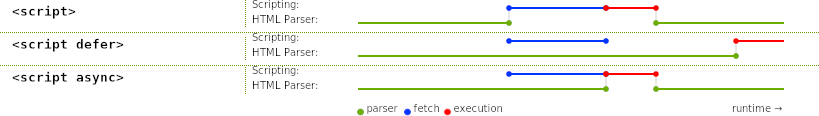
\includegraphics[width=0.8\textwidth]{scripts.png}
\caption{Scripts}
\label{figure:script_loading}
\end{center}
\end{figure}


The async and defer attributes do not apply to inline scripts.
The HTML standard states that "scripts may specify defer or async, but must not specify either unless the src attribute is present."\footnote{\url{https://html.spec.whatwg.org/multipage/scripting.html} [11.08.2021]}

Since inline scripts do not contain a src attribute because the source of the script is inside the script tags and not external, the async and defer attributes are not applicable.


% https://blog.logrocket.com/5-tricks-to-eliminate-render-blocking-resources/
%- The defer attribute is recommended for scripts that need the DOM, but you want to begin to download them before the document loads, without making them a render blocking resource.
%- You should also use defer rather than async if the document order is important — for instance, when consecutive scripts depend on each other.



% [Transition]

HTML, CSS and JS are now processed and the CRP proceeds to build the render tree as described below.

% [More stuff]

% add this? preload scanner
% https://developer.mozilla.org/en-US/docs/Web/Performance/How_browsers_work
%- Though the browser's preload scanner hastens this process.

% Grigorik Conference Talk https://www.youtube.com/watch?v=PkOBnYxqj3k&ab_channel=IlyaGrigorik
% And slides https://www.igvita.com/slides/2013/fluent-perfcourse.pdf
%- Asynchronous pattern:
	%- Not the same as async/defer tag
	%- Will fetch JS asynchronously
	%- Uses IIFE which creates a new script tag in the HTML with attribute async
	%see chapter X how Google Analytics is doing this.


% add this? https://web.dev/render-blocking-resources/
%Lighthouse flags resources as render blocking when:
%A <script> tag that:
%Is in the <head> of the document.
%Does not have a defer attribute.
%Does not have an async attribute.


% add this? resource hints
% https://blog.logrocket.com/using-resource-hints-to-optimize-performance/



% ------------------------------------------------------------


\paragraph{Building the Render Tree} % korrigiert

As described above, both HTML and CSS are rendering blockers because they prevent the page from rendering.
Rendering can only occur once the render tree is available.
The render tree is the combination of DOM and CSSOM and captures all visible content with their styles to be displayed on the screen.
If an element has a CSS property like \verb|display: none;|, it is not displayed in the render tree \cite{2019GrigorikRenderTree}.

The calculated render tree is then used for the layout of the content on the page.


% add this ? Check again when chapter about WPT metrics is done
% 2014 Hogan https://designingforperformance.com/
%Chapter 2
%- Start Render Metric in WPT


% ------------------------------------------------------------

\paragraph{Layout} % korrigiert

In the layout process, the position and size of the nodes are calculated from the render tree.
New layout calculations or re-flows are triggered as soon as the screen area changes, e.g. by rotating the device or resizing the window, or when the DOM and the render tree change \cite{2021MDNHowBrowsersWork}.

Once the layout is resolved, the browser continues painting pixels on the screen.

% add viewport? The projection area is dependent and defined by the viewport

% https://developer.mozilla.org/en-US/docs/Web/Performance/Critical_rendering_path
%- The viewport meta tag defines the width of the layout viewport, impacting the layout.
%- Without it, the browser uses the default viewport width, which on by-default full screen browsers is generally 960px. On by-default full screen browsers, like your phone's browser, by setting <meta name="viewport" content="width=device-width"



% ------------------------------------------------------------


\paragraph{Paint} % korrigiert

Finally, the browser can paint the content on the screen.
When content changes, browsers are optimized to redraw only the affected areas on the screen \cite{2021MDNCRP}.

% add This ?

% metrics ?
% How Browsers Work https://developer.mozilla.org/en-US/docs/Web/Performance/How_browsers_work
%-> First Meaningful Paint
%- Time to Interactive

% above the fold?
% https://gtmetrix.com/blog/how-to-eliminate-render-blocking-resources/
%- Above the fold: “Above-the-Fold” refers to the area that the visitor normally sees on a website before scrolling down to see the rest of the content. 

% performance question?
% https://blog.logrocket.com/how-css-works-parsing-painting-css-in-the-critical-rendering-path-b3ee290762d3/
%- Paint: It’s important to remember that some CSS properties can have a larger impact on the page weight than others (for example, a radial-gradient is much more complex to paint than a simple color).



% ------------------------------------------------------------


% add this ?
% [Continuos Loop, 60 frames per second]
% [Compositing ?]


% ------------------------------------------------------------

\subsection{The Website Loading Process: Conclusion} % korrigiert

The loading process of a website is complex and multi-layered.
The goal of this section was to provide a general understanding and idea of it.
For this purpose, the loading process is divided into three components: The front-end, the back-end, and the network.
We have seen that within the network component there are several mechanisms to ensure a reliable and secure connection between the front-end and the back-end.
Within the front-end component, the Critical Rendering Path describes the steps that the browser must take to retrieve and render a website.

% [Link to next section]

It is important to have a general understanding of the loading process of a website in order to understand web performance metrics.
Before discussing web performance metrics in section \ref{section:web_performance_metrics}, methods for measuring them are described in the next section.


% add ?
% give some links and references to optimization

% [Optimizations]

% Grigorik Conference Talk https://www.youtube.com/watch?v=PkOBnYxqj3k&ab_channel=IlyaGrigorik
% And slides https://www.igvita.com/slides/2013/fluent-perfcourse.pdf
%- Optimize the critical rendering path!
%-> styles at the top, scripts at the bottom best practice
% - Different browsers implement different logic for when, and in which order, the individual resource requests are dispatched. As a result, the performance of the application will vary from browser to browser. 2013 Grigorik ch 10

% 2014 Hogan https://designingforperformance.com/
%- Optimizations of CRP:
%- media types and queries on css resources, which makes them non-blocking
%- Load JS efficient
%- Priotize requests for above the fold
%- etc. % Do i need to explain this ??
%Chapter 4:
%CSS and JavaScript Loading:
%- Rules:
%- Load CSS in head
%- CSS blocks rendering
%- Load JS at bottom of the page
%- Load Async
%- JS blocks DOM construction, because browser knows that content from script tag may change Render Tree
%- async tag will execute script once its ready, but order is not berücksichtigt
%- Anything that loads late and changes UI can cause layout shifts
%- 3rd party scripts: Need additional DNS lookup, should not be single point of failure

% https://developer.mozilla.org/en-US/docs/Web/Performance/Critical_rendering_path
%- Optimizing for CRP

% https://medium.com/@luisvieira_gmr/understanding-the-critical-rendering-path-rendering-pages-in-1-second-735c6e45b47a
%- Optimizing

% Grigorik Conference Talk https://www.youtube.com/watch?v=PkOBnYxqj3k&ab_channel=IlyaGrigorik
% And slides https://www.igvita.com/slides/2013/fluent-perfcourse.pdf
%- Async all the things! nice image about async attribute
%- Optimizing DOM:
	%- Minify HTML
	%- Compression
	%- Cache in Browser
%- Unblocking CSS:
	%- Media queries: for responsive design
	%-> Move media queries to separate file
	%- <link rel="stylesheet" href="style-print.css" media="print">
	%-> Will not block rendering
%- Optimizing JS:
	%- Minify, compress, cache
	%- JS is parser blocking
	%- Script tag blocks DOM construction
	%- For external JS, browser waits until JS is fetched and executed
	%- CSS blocks rendering and JS execution
	%- Load and execute script after page is loaded
	%- Page is loaded: Browser fires onload event
	%- Async attribute:
		%- <script src="a.js" async></script>
		%- Does not block CRP (DOM construction, CSSOM)
	%- Inline script blocks CSSOM unless included before CSS request
%- General Strategies:
	%- Minify, compress, cache (HTML, CSS, JS)
%	- Minimize use of render blocking resources (CSS):
	%	- Media queries
		%- Inline CSS
%	- Minimize use of parser blocking resources (JS):
	%	- Defer JS execution
		%- async attribute
%	-> Minimize Bytes
	%-> Reduce critical resources
	%-> Shorten CRP length
	
% 2013 Grigorik
%- Browser optimizations...

% 2016 Witt code talks
%- tools available:
%- Profiling: GTMetrix, WebPageTest, PageSpeed Insigths
%- Inlining and Optimization: Critical, PostCSS, processhtml
%- Minification and Compression: Goole Closure, tinyPng, Uglifycss and cssmin

% 2014 Hogan https://designingforperformance.com/
% Chapter 2 The Basics of Page Speed - How Browsers Render Content:
%- Browsers try to parallelize requests for content
%- Requests: Optimizing size and amount of requests has big impact on performance, e.g. get all images in one requests using Sprites

%Page Weight is somewhat important:
%- Sum of all file sizes
%- Averages in httparchive, which i also used in one approach % https://httparchive.org/reports/state-of-the-web?start=latest

%Other Impacts on Page Speed
%- "environmental factors"
%- Geography, CDNs
%- Network
%- Browser

% 2016 Witt code talks
%- Possible Improvements:
%- HTTP2
%- Avoid redirects
%- Caching headers
%- CDNs
%- Single Page Apps

% add this ??
% [JavaScript Parsing]
% https://medium.com/reloading/javascript-start-up-performance-69200f43b201


% --------------------------------------------------------------------------------------------------------
% --------------------------------------------------------------------------------------------------------


\section{Measurement Methods} % korrigiert
\label{section:measurement_methods}

In this section, I will discuss what methods and techniques are available to measure the performance of a website.
The two most important methods are synthetic monitoring, as described in section \ref{subsection:synthetic_monitoring}, and Real-User Monitoring, as discussed in section \ref{subsection:RUM}.

A concrete example is given for each of the methods.
WebPageTest as a synthetic monitoring solution in section \ref{subsection:webpagetest},
and Google Analytics as a Real-User Monitoring tool in section \ref{subsection:google_analytics}.

Both are used in the controlled experiment that addresses the research question, as explained in chapter \ref{chapter:approach}.
After this section on measurement methods, I describe which performance metrics are measurable.

% [Link to Research Question] ??

% ----------------------------------------------------------------------------------------------


\subsection{Synthetic Monitoring}
\label{subsection:synthetic_monitoring}


\subsubsection{The "Synthetic" Aspect in Synthetic Monitoring} % korrigiert

As the name implies, synthetic monitoring is a measurement method performed in an artificial, laboratory-like, synthetic environment.
Test agents simulate real users and are configured to run a browser, load the observed website, and collect performance data in the process.
Synthetic monitoring does not take into account real user traffic \cite{2015Cito}.

%TODO
Performance data can be collected via common performance APIs as described in section X.
In addition, user-centric metrics such as Speed Index can be calculated through video recording and analysis (see Section X) \cite{2021Wingerath}.

Synthetic monitoring controls many possible configurations and variables of the test agent (client), such as location (geography), network conditions, device type, browser version, and so on \cite{2021MDNRUMvsSynthetic}.
So the tester has control over many variables that affect performance, and can also change these variables to test how they affect performance.

The controlled environment enables the collection of performance data for a specific configuration, such as the location of the test agent or browser version, which can help identify issues with specific user segments.
For example, a test could check the performance of all users using Firefox on macOS in Germany \cite{2009Croll}.

In addition to defining the technical configuration, such as browser version or network conditions, the tester can also define artificial user journeys to simulate real user behaviour \cite{2021Wingerath}.

A feature of the controlled environment provided by synthetic monitoring is that the measured data and test results are relatively consistent with little variability, providing a performance baseline for the site being monitored and facilitating performance optimization \cite{2013Meenan}.


\paragraph{Synthetic Monitoring is not about Real Users} % korrigiert

Synthetic monitoring does not collect data from real users, as traffic on the website is generated artificially.
Real user behaviour is approximated by simulating users, e.g., by prescribing user paths.
Measured performance data does not necessarily reflect the actual user experience, and the tester should not assume that "synthetic results are like real-user metrics" \cite{2016Viscomi}.

Capturing the wide variety and diversity of real users, such as the pages visited, the user's general configuration such as CPU, GPU, and memory performance, what data is stored in the browser cache and what browser version is used, screen size, operating system, and network connection, to name a few, is difficult to represent in synthetic monitoring \cite{2013Meenan}, \cite{2013Grigorik}.
The selected test configuration in synthetic monitoring only reflects a specific use case and can only approximate what a user with a similar configuration might experience \cite{2016Viscomi}.
In short, synthetic monitoring test results "are synthetic and therefore not representative for actual user data" \cite{2021Wingerath}.


\subsubsection{The "Monitoring" Aspect in Synthetic Monitoring} % korrigiert

Synthetic monitoring can be automated and used to monitor a system's performance in real time and provide up-to-date reports for the system administrator \cite{2021MDNRUMvsSynthetic}.
Monitoring makes it possible to check site availability around the globe \cite{2009Croll},
detect performance problems before users notice them \cite{2013Grigorik},
and is generally useful for continuous "health checks" of the running system \cite{2021Wingerath}.

Since each website can be tested synthetically, it is possible to compare the performance data of several competitors \cite{2009Croll}.


% [Tools]

There are many synthetic monitoring tools (see for example \cite{2016Kaur} for a list of tools). %TODO add online sources
\textit{WebPageTest} is one of them and is discussed in section \ref{subsection:webpagetest}.


% [Transition]

%TODO
As described in Section X, the performance of an online store correlates with sales.
Synthetic monitoring enables the collection of performance metrics independent of real user behaviour.
Real user behaviour is not measured in synthetic monitoring.
Since only real users are able to generate revenue, synthetic monitoring cannot detect correlations between user satisfaction (and revenue) and performance (as described in Section X) \cite{2021Wingerath}.

Understanding the correlation between user satisfaction and website performance requires Real-User Monitoring (RUM).
RUM enables the collection of data from each real user.
RUM will be covered in section \ref{subsection:RUM}.

Before that, a common synthetic monitoring tool, \textit{WebPageTest}, is briefly discussed.


% cut out google lighthouse completely ?
%- Google Lighthouse

% add waterfall ?
% 2021 Wolle blog post https://medium.baqend.com/mobile-site-speed-measurement-best-practices-ff4a3f91b003
%- waterfall diagram contains timing information on when the individual resources were requested, from which domain and over what kind of connection each of them was served, and how long transmission took

% 2016 Viscomi
%- synthetic tools are deliberately designed to focus on the performance of a web page under strict conditions that are otherwise highly volatile in real-user performance

% 2021 Wolle blog post https://medium.baqend.com/mobile-site-speed-measurement-best-practices-ff4a3f91b003
%- Modern tooling also tells you when the browser was actually doing useful work (e.g. rendering) and when it was idle and waiting for loads to finish


% --------------------------------------------------------------------------

\subsection{WebPageTest} % korrigiert
\label{subsection:webpagetest}

%TODO
As will be discussed in Section X, I will use a synthetic monitoring tool to measure and compare performance metrics in the context of a controlled experiment, which will help answer the research question.
There are many synthetic monitoring tools available. 
The tool used is WebPageTest (WPT) and will therefore be briefly discussed here.

"WebPageTest is a web performance tool providing deep diagnostic information about how a page performs under a variety of conditions."\footnote{\url{https://docs.webpagetest.org/} [11.08.2021]}
WPT was made available to the public in 2008 and was acquired by Catchpoint in September 2020\footnote{\url{https://www.catchpoint.com/webpagetest-joins-catchpoint} [04.08.2021]}.
WPT is open source\footnote{\url{https://github.com/WPO-Foundation/webpagetest} [04.08.2021]} and offered as a free web service\footnote{\url{https://www.webpagetest.org/} [04.08.2021]} and can be used by anyone.

Some of the key features of WPT are that it measures and provides a variety of metrics (see Section X), it facilitates saving and sharing performance test results, it provides waterfall graphs, a breakdown of the website's content, or even film strips and video recordings of the loading process \cite{2016Viscomi}.

The main goal of WPT is to "provide detailed information to developers about the loading performance of their pages in a realistic end user environment" \cite{2016Viscomi}.

WPT is widely used, "the leading web performance tool in the world today" \cite{2016Viscomi}, and an "indispensable power tool in your web performance toolkit" \cite{2013Grigorik}.

% add this ??
% API: 
% RESTful
% programatically run tests and fetch results from WebPageTest
%This will allow integration with an existing web development pipeline, as well as the automation of the whole % process of running a test and reading its results once the test is complete


\subsubsection{Configuration} % korrigiert

WPT is highly configurable and allows performance testing for almost any desired configuration.
One of the key configuration options is that testing can be performed from multiple geographic locations, with test sites provided by over fifty companies and individuals \cite{2016Viscomi}.

Other configurations include, for example, the possible selection of different devices and browsers, e.g., Chrome emulation from an iPad in Taiwan; the setting of Repeat View, which instructs the browser to load the website not only the first time but also the second time, which provides insight into the caching setup of the website; and the throttling of the network, e.g., whether to use DSL or 5G.

The configuration options give the investigator control over many variables that can affect performance. 
The settings used for the experiment to answer the research question are explained in Section X.

% 2011 Grigorik https://hpbn.co/primer-on-web-performance/
% the browser runs within a virtual machine and can be configured and scripted with a variety of connection and browser-oriented settings


\subsubsection{Private Instances} % korrigiert

The public WPT instance is reliable and configurable, but depending on the test location, it can also lead to waiting times because other people are also using it.
Also, the public WPT instance can only access and thus test and evaluate publicly accessible websites \cite{2016Viscomi}.
There are also daily limits on how much testing can be done.

Private WPT instances help to counteract the problems described.
Since WPT is open source, it is possible to create and use your own version of WPT.
Private instances allow unlimited testing and give the tester full control over the infrastructure.
An additional and only available feature for private instances are bulk tests.
Bulk tests allow a list of URLs to be passed to WPT for processing.
In Section X, I describe how this feature can be used to test the same URL multiple times and how private instances are set up and used.

% [Transition]

WPT captures a variety of performance metrics.
What performance metrics are is described in Section X, and what metrics are available through WPT in Section X.
The next section discusses another important method for measuring web performance, Real-User monitoring.


% add this ?
% [Architecture]

% 2016 Viscomi
% two types of components: a server and the test agents.
% server provides the web interface and API; it also queues and schedules the work for the individual test agents.
% After the agents have completed a test, it recieves the results and displays them.

%The second type of component is the test agents, which actually load the page in a browser and gather metrics as it loads. These test agents might be desktop browsers running on Windows, Safari running on a iOS device, Android devices running Chrome, or remote ones on another WebPageTest instance
% The test agents poll the server for work, measure the page load, and then when the test completes, upload the measurements and any screenshots it took

% add ??
% Waterfall
% Grades
% See in performance tab for details about grades and optimization techniques
% Differnce between conenction view and request view as described in section X.

% 2014 Hogan ch 2
%- A waterfall chart such as Figure 2-2 shows you how much time it takes to request the contents of a page, such as CSS, images, or HTML, and how much time it takes to download this content before displaying it in a browser.
% 2011 Grigorik Analyzing the Resource Waterfall in https://hpbn.co/primer-on-web-performance/
% [Waterfall: Resource Waterfall and Connection View]


% ----------------------------------------------------------------------------------------------
% ----------------------------------------------------------------------------------------------


\subsection{Real-User Monitoring} % korrigiert
\label{subsection:RUM}

As the name suggests, Real-User Monitoring (RUM) is about collecting and measuring data from real users who visit the website.
Unlike synthetic monitoring, which artificially generates website traffic and only approximates the performance experience of real users, RUM data relies on real user traffic and captures data directly from each user's browser. 
RUM measures performance as experienced by users \cite{2021MDNRUMvsSynthetic}.


\subsubsection{The Page Tagging Technique in RUM} % korrigiert

% [Page Tagging]

As described in Section X., page tagging is a technique that instruments the user's browser to collect data and report it to an analytics server.
RUM is based on page tagging, i.e., a JS code snippet ("tracking code") that is loaded into the user's browser.
Once this tracking code is loaded and executed in the browser, it collects data and sends it back to an analytics service.
If the user blocks JS or the script cannot be downloaded for other reasons, RUM will not work.
Once the data arrives at an analytics service, it must be stored and an interface must be provided for the analyst to query the data and gain insights, such as by providing a dashboard \cite{2021Wingerath}.

Since RUM relies on the JS code, the very first opportunity to measure data is when this JS code has been downloaded and executed.
Anything that happens before that step is invisible to the tracking script, and therefore invisible to the analyst.
Meenan notes that about 20\% of the loading process is outside the RUM measurement range and that "getting a reliable start time for measurements from the real world has been the biggest barrier to using RUM" \cite{2013Meenan}.

Another facet of RUM is that the measurement of data should ideally have as little impact as possible on the site rendering process, and network capacity should not be taken up by RUM scripts and block resources of the CRP \cite{2021Wingerath}.
One of the research questions of this paper is whether RUM, as a page marking technique, slows down the observed website.
The evaluation of the controlled experiment to answer this question shows that RUM...., as described in section X. %TODO add conclusion of evaluation here

% [Diversity of Users and Data]

RUM is independent of the user's setup or environment and collects data for all active users:
Regardless of the user's device, browser, network conditions, or geographic location, RUM collects data as long as the measurement script is loaded into the user's browser \cite{2021MDNRUMvsSynthetic}.
So the RUM data represents each individual user experience \cite{2016Viscomi}.

Due to the diversity of users and the unique environment of each user, RUM data tends to be more diverse and heterogeneous than data collected through synthetic monitoring \cite{2013Meenan}.


\subsubsection{RUM Measures Behaviour of Real Users} % korrigiert

% [E-Commerce Background]

As discussed in section X, website performance and user satisfaction are directly related.
An important component of RUM is not only the collection of performance metrics, but also the measurement of user behaviour, e.g., how the user interacts with the website and where he or she clicks \cite{2021Wingerath}.
In an e-commerce context, user behaviour questions are of interest, such as whether a new campaign changes user behaviour as expected or where users leave the check-out process \cite{2021Wingerath}, \cite{2021MDNRUMvsSynthetic}.

RUM enables the combination of collected metrics with user behaviour and business KPIs and can answer questions such as whether and how website performance affects user behaviour, e.g. whether users buy more or less depending on the speed of the website \cite{2021Eggplant}.
Thus RUM is not only important to understand user behaviour, but also to optimize the website and increase sales.
With techniques such as cookies (see section X.), it is also possible to track user behaviour not only for one page visit, but over a series of website visits, resulting in even more detailed insights about the visitor \cite{2021Wingerath}.

% [Tools]

There are several RUM tools and JS libraries, such as Boomerang from Akamai.\footnote{\url{https://github.com/akamai/boomerang} [23.06.2021]}
The main player, Google Analytics, is discussed in more detail in section \ref{subsection:google_analytics}.

% SpeedKit ?

% [Transition]

Google collects RUM and browser data from Chrome users who have consented to it.
The data is accessible via the Chrome User Experience Report (CrUX) and is discussed below.


% add this here?
% [Performance Data]

%Which data and metrics RUM can collect and measure is discussed in greater detail in section X.
%A part from metrics exposed by Web APIs or own implementations
%RUM can also gather data about the users device, operatins system or geographic location. %cite 2015 Cito
%The performance data and timings are exposed through a variety of APIs which the JS tracking code has access to.

% 2013 Grigorik https://hpbn.co/primer-on-web-performance/
%- APIs to measure real users (will be discussed in metrics chapter):
%- Navigation Timing
%- Resource TIming
%- User TIming
%- The combination of Navigation, Resource, and User timing APIs provides all the necessary tools to instrument and conduct real-user performance measurement for every web application

% Cito
%- Real-User Monitoring leverages browser APIs to collect data specific to each end-user transaction

% 2021 Wolle blog post https://medium.baqend.com/mobile-site-speed-measurement-best-practices-ff4a3f91b003
%- Collected information includes various timers to capture network and rendering performance
%- To also capture details about the user’s device and browser or on the referring website over which the user arrived, the user agent string and other data artifacts are collected along with the values obtained from the Navigation and Performance Timing APIs


% [Business Data]

%conversion rates etc.

% --------------------------

\subsubsection{Chrome User Experience Report (CrUX)} % korrigiert

The Chrome User Experience Report (CrUX) is a RUM method implemented by Google that collects real user data from Chrome users.
Once the Chrome user gives consent, data collection can begin and does not need to be set up.
The CrUX only collects data from Chrome users and is therefore not a complete sample of the Internet user population, as it does not collect data from users who browse the Internet using Firefox or Safari, for example \cite{2021Wingerath}.
The collected data is available via Google's PageSpeed Insights, the CrUX Dashboard or the BigQuery and CrUX API \cite{2021Crux}.

CrUX is important in that it collects data from real users across millions of websites and measures user data such as device types, but also performance metrics such as Core Web Vitals (see section \ref{subsubsection:core_web_vitals}).
CrUX therefore provides insight into how a broad spread of real users experience the website and also enables direct comparison with competitors \cite{2020Viscomi}.

% ----------------------------------------------------------------------------------------------


\subsection{Google Analytics} % korrigiert
\label{subsection:google_analytics}

% [Why]

As will be explained in Section X, I will use a RUM tool to measure and compare performance metrics in the context of a controlled experiment, which will help answer the research question.
There are many RUM tools available. 
The tool used is Google Analytics (GA) and will therefore be briefly discussed here.

% [Definition]

GA is a RUM solution that helps to "determine how successful your site is at turning users into customers".\footnote{\url{https://marketingplatform.google.com/about/resources/analytics-product-overview/} [05.08.2021]}

% [Short History]

GA is by far the most widely used analysis tool today.\footnote{\url{https://w3techs.com/technologies/overview/traffic_analysis} [05.08.2021]}
The first version of GA was initially developed by Urchin Software Corporation and acquired by Google in 2005.
The second version, Classic GA, was released in 2007.
The third version, Universal Analytics, was released in 2013 and the latest version, Google Analytics 4, was released in 2020.
Each version improved the quality of measured data and integration with other Google products \cite{2021Franco}.

% [Features]

GA offers a wide range of functions.\footnote{\url{https://marketingplatform.google.com/about/analytics/features/} [05.08.2021]}
Worth mentioning, for example, is analytical intelligence, a system that answers specific questions asked by the tool's users by extracting answers from the data;
a variety of reports, such as real-time reports or conversion reports;
or general data analysis, visualization and monitoring, such as with custom segmentation.

GA also tracks a number of web performance metrics.
What these are and how they are calculated is described in section \ref{subsubsection:ga_metrics}.

% [How it works]

GA is a RUM method and therefore relies on the page tagging technique, as explained in Section X.
Some examples and aspects of how to integrate the GA tracking script into the monitored website are explained in Section X.

% Kessler 2012 p. 581

% ----------------------------------------------------------------------------------------------

%TODO add this ??

% \subsection{Log Files and Surveys}

% [tbd]

% Other methods are surveys and log file analysis.

% 2021 Wolle blog post https://medium.baqend.com/mobile-site-speed-measurement-best-practices-ff4a3f91b003

%Log analysis:
%- concerned with technical performance in the backend
%- generates insights from the data that is already available from the application server, proxy, or content delivery network (CDN)
%- TTFB
%- Server logs typically only reflect the time it took to send the first response, not until the client actually started receiving it
%- Analyzing logs from application servers, CDNs, or proxies is a reasonable first step to discover potential bottlenecks, but it only covers the server side and does not provide any information on client-side processing in general or rendering performance in particular


%Surveys:
%- directly ask the users for their opinions
%- direct approach to understanding whether or not users are satisfied with website performance: Just ask them for their opinion
%- online surveys or by offering some sort of price or chance to win a competition in exchange for the users opinions. 
%- Other options include actual interviews or monitoring users in a lab setting to find out how they react while surfing on the website.
%- they only cover a small sample of the user base and therefore may be subject to a certain selection bias
%- user perception can be highly inaccurate
%- Getting reliable info from user surveys is therefore no trivial task
%- some forms of surveys (e.g. lab experiments) can be relatively expensive to conduct in comparison to some of the fully automated alternatives for collecting information
%- are great for collecting qualitative feedback on the user experience, but are not suitable for gathering quantitative measurements



% ----------------------------------------------------------------------------------------------

\subsection{Measurement Methods Conclusion} % korrigiert

There are two main complementary techniques to measure the performance of a website: synthetic monitoring and Real-User Monitoring (RUM) (table \ref{table:synthetic_monitoring_rum_comparison}).

Synthetic monitoring measures the performance of a website in a controlled environment using test agents and is particularly useful for finding a baseline for website performance and for continuous monitoring and health checks.
Performance as perceived by end users can only be approximated, as it is not captured by synthetic monitoring.

RUM collects data from each user who visits the website and reports it back to an analytics server.
RUM is particularly useful when multiple metrics are combined, such as performance and business metrics, to analyse user behaviour.
On the other hand, if no user visits the website, RUM does not collect any data.

Other performance measurement methods such as CrUX and surveys provide browser-specific or quality data and complement the analysts' toolkit.

\begin{table}[h]
	\small
	\centering
	\begin{tabular}{ | c | c | }
	\hline
	Synthetic Monitoring \cellcolor{lightgrey} & RUM \cellcolor{lightgrey} \\
	\hline
	Artificial test agents & Real users \\
	\hline
	Controlled configuration & No control over the configuration \\
	\hline
	Approximates real user data & Collects real user data \\
	\hline
	For monitoring & Links user behaviour to business KPIs \\
	\hline
	\end{tabular}
	\medskip
	\caption{Comparison of Synthetic Monitoring and RUM}
	\label{table:synthetic_monitoring_rum_comparison}
\end{table}

% [Metrics, Transition]

Measurement methods such as synthetic monitoring or RUM can measure metrics to map website performance or business success to some kind of value or number.
As discussed in section X, there are a variety of web analytics metrics to measure any business-related aspect of the website, such as conversion or bounce rates.

Website performance can also be measured using the methods described above.
There are a variety of web performance metrics.
What they are, how they have evolved, and what they monitor will be covered in the next section.


% ----------------------------------------------------------------------------------------------------
% ----------------------------------------------------------------------------------------------------

\section{Web Performance Metrics} % korrigiert
\label{section:web_performance_metrics}


% [Performance Metrics]

As discussed in Section X., web analytics (or business or non-performance) metrics collect data on many different aspects of an online business, such as how many visitors the website has or what the conversion rate is.
A number of specific metrics are required to measure \textit{performance}, such as the speed of the website and how users perceive the website's performance.
Performance metrics are created to measure various aspects of a website's performance and are discussed in this section.


% [Quantification and Analysis]

Performance metrics make performance quantifiable because the metrics reflect performance in numbers.
Once performance is mapped into numbers, they can be compared with each other, e.g., over time, after a change in the measured application, or with a competitor's numbers \cite{2021MDNMeasuringPerformance}.
By quantifying performance, metrics facilitate the analysis of website traffic.
Specific metric values can be used as targets for goal achievement and are therefore an important tool for improving websites \cite{2009Jansen}.
Ideally, metrics are precise and serve as objective criteria for evaluating the measured website \cite{2019WaltonUserCentric}.


% [Outline]

As with web analytics metrics, there are several ways to structure and categorize performance metrics.
One way to bring order to performance metrics is to distinguish between \textit{Navigation Timing Metrics} (section \ref{subsection:navigation_timing_metrics}), which measure elapsed time for specific processes and navigation steps from the CRP, and \textit{User-Centric Performance Metrics} (section \ref{subsection:user_centric_performance_metrics}), which approximate user-perceived performance through visual analysis.
Both classes of metrics are discussed below.

Before that, I'll discuss \textit{Page Weight} (section \ref{subsection:page_weight}), a metric that characterizes the size of a website.
The benefits of \textit{Custom Metrics} and why they are important are discussed in section \ref{subsection:custom_metrics}.

As described in section X, WebPageTest and Google Analyitcs are common tools for synthethic monitoring and RUM, respectively, and will be used in the controlled experiment described in chapter X.
What performance metrics they measure is described in section \ref{subsection:wpt_ga_metrics}.


% [Link to Research Question] ??


% add this ?
% https://speedcurve.com/blog/rendering-metrics/
%- Metrics quantify behavior
%- we're trying to capture the behavior of a website in terms of speed and construction
%- statistics about how the site is built such as number of HTTP requests, size of stylesheets, and DOM depth
%- Speed is tracked by time-based metrics that capture when things happen during the user's experience with the website: start render, DOM interactive, page load, etc. 


% add this ?
% Summary / Metrics Taxonomy
% 2019 Enghardt
%"metrics as well as experiments have to realistically reflect possible performance improvements for actual users"

% [Metrics and KPIs]
% 2015 Bekavac


% add this?
% No official definitions, lack of definitions (enghardt)
% Still there are informal standard
% Implementation can vary between tools who measure metrics

% -----------------------------------------------------------------------

\subsection{Page Weight} % korrigiert
\label{subsection:page_weight}

A naive approach to quantifying a website is to measure its size and the resources required to build it.
Page weight can be used as a performance measure because the performance of a website depends on its size, especially when combined with network conditions such as download speed and latency.
The more bytes that need to be transferred over the network, the longer it takes for the website to build, and the longer the wait for the user.
The situation is similar for requests: the more requests are required, the more connections have to be established, which in turn takes more time.

A website consists of several resources, such as HTML files, fonts, script files or images (see table \ref{table:website_resources}).
The page weight describes the number of bytes and requests retrieved for each resource type. % compare cite HTTP Archive

\begin{table}[h]
	\small
	\centering
	\begin{tabular}{| c | c | c | c | }
	\hline
	HTML & CSS  & JS & Fonts \\
	\hline
	Images & Videos & Others & (Total) \\
	\hline
	\end{tabular}
	\medskip
	\caption{Types of resources of a website}
	\label{table:website_resources}
\end{table}

Page weight is an initial assessment of a website's performance.
It is mainly useful for comparison with median values of other websites, but has little to no significance and meaning for evaluating the performance of a website.
To gain more meaningful insights into a website's performance, other metrics are needed, such as navigation timing metrics, which are discussed in the next section.
As will be described in section X, the idea of page weight is used to create a test page with an average page weight value.


% -----------------------------------------------------------------------


\subsection{Navigation Timing Metrics} % korrigiert
\label{subsection:navigation_timing_metrics}

Navigation timing metrics show the elapsed time within the website loading process, such as the network navigation process and CRP (see section \ref{section:website_loading_process}).
They are computed and derived from a set of standardized Web APIs.

In the following, I will briefly explain the nature of Web standards and recommendations (section \ref{subsubsection:web_standards}).
I will then discuss performance-related specifications and the metrics they provide (section \ref{subsubsection:w3c_performance_specifications}).


% -------------------------

\subsubsection{Web Standards} % korrigiert
\label{subsubsection:web_standards}

Web standards are documents that describe the technology used to build the WWW \cite{2021MDNWebStandards}.
These documents, also called specifications, are maintained by various groups and organizations.
There are several organizations that create and maintain standards for different areas and technologies of the Web.
Such organizations include the WHATWG, which maintains the living HTML standard\footnote{\url{https://whatwg.org/} [07/11/2021]}, or Ecma International, which maintains the specification for JS.\footnote{\url{https://www.ecma-international.org/} [11.07.2021]}.

The World Wide Web Consortium (W3C) is an organization that maintains various standards for the WWW, including specifications for performance measurement\footnote{\url{https://www.w3.org/} [11.07.2021]}, which I will discuss below.


\paragraph{W3C} % korrigiert

% [What is W3C]

The W3C was founded in 1994 by Tim Berners-Lee with the goal of bringing together "representatives from many different technology companies to work together on the creation of web technology specifications" \cite{2021MDNWebStandards}.
The W3C manages and publishes documents that describe and define web technologies such as DOM, SVG or CSS \cite{2021W3CFAQ}.


% [Recommendation Process]

The creation of a document or specification follows a "recommendation track" that describes the hurdles a document must overcome to move from an idea to a final recommendation and web standard that browser vendors implement as concrete APIs \cite{2020W3CProcessDocument}.
The stages of the recommendation process are described by the "maturity levels" of the document and are as follows:
First Public Working Draft (FPWD) $\,\to\,$ Working Draft (WD) $\,\to\,$ Candidate Recommendations (CR) $\,\to\,$ Proposed Recommendation (PR) $\,\to\,$ W3C Recommendation (REC) \cite{2015W3CProcessDocument}.
W3C recommendations are considered web standards \cite{2021W3CFAQ}.

%TODO maybe draw some nice graphic for the recommendation track ?


\paragraph{Web Performance Working Group} % korrigiert

% [Introduction]

Within the W3C there are several groups, each dealing with a specific topic in the WWW universe \cite{2021W3CWorkingGroups}.
Founded in 2010, the Web Performance Working Group is a group whose mission is to "provide methods to measure aspects of application performance of user agent features and APIs" \cite{2021W3CWebPerformanceWorkingGroup}.

% [Specs]

The Web Performance Working Group publishes and maintains a number of documents that address performance measurement, such as High Resolution Time, Navigation Timing, and Page Visibility \cite{2021W3CWebPerformanceWorkingGroupPublications}.
The published papers that are particularly relevant to performance measurement are discussed below.

% add this ?
% https://www.w3.org/2021/02/webperf.html
%- Working Groups push new recommendations and invent them
%Web Performance Working Group is responsible:
%- Measurement
%- Scheduling
%- Adaptation
%-> Important is Measurement

% https://w3c.github.io/perf-timing-primer/#dfn-time-origin
%- attempt to address the concern about lacking insight into how or why certain stages of the request-response cycle have taken as much time as they have

% others, not important for metrics:
%- Beacon
%- Cooperative Scheduling of Background Tasks
%- Device Memory
%- Reporting
%- Network Error Logging

% -----------------------------------

\subsubsection{W3C Performance Specifications}
\label{subsubsection:w3c_performance_specifications}


\paragraph{High Resolution Time} % korrigiert

There are two versions of High Resolution Time.
High Resolution Time Level 2 has the maturity level of a W3C Recommendation and was released in November 2019 \cite{2019W3CHRTime2}.
The newer specification, simply High Resolution Time, is a current working draft \cite{2021W3CHRTime}.
The High Resolution Time specification does not directly define performance metrics, but serves as the basis for other specifications for measuring and recording time values.

% [Date/Clock Issue]

Prior to High Resolution Time, time values were calculated using the ECMAScripts Date object, which represents time in milliseconds since January 1, 1970 UTC \cite{2021Ecma}.
This time definition is inaccurate with respect to time shifts and system clock adjustments.
It is possible that the time values derived from the Date object do not increase monotonically or sometimes even decrease.

High Resolution Time solves these problems and provides monotonically increasing time values, sub-millisecond resolution, and a starting value that refers to the beginning of the navigation process on the website instead of the year 1970, making it easier to understand and calculate timestamps and intervals \cite{2021W3CHRTime}.
The specifications described below use the precise time information provided by High Resolution Time.

% High Resolution Time defines a Performance interface, which exposes a function $now()$, which returns the current time.


% add this ?
% https://developers.google.com/web/updates/2012/08/When-milliseconds-are-not-enough-performance-now
%- performance.now() is a measurement of floating point milliseconds since that particular page started to load
%-> the performance.timing.navigationStart timeStamp to be specific
%- number stays relative to the page because you'll be comparing two or more measurements against eachother


% [DOMHighResTimeStamp]

% https://www.w3.org/TR/hr-time-3/
%- type definition
%-  used to store a time value in milliseconds, measured relative from the time origin, shared monotonic clock, or a time value that represents a duration between two DOMHighResTimeStamps
	
% https://developer.mozilla.org/en-US/docs/Web/API/DOMHighResTimeStamp
%- type
%- double
%-  store a time value in milliseconds,  accurate to 5 microseconds
%- describe a discrete point in time or a time interval


% [Performance Interface]

% https://www.w3.org/TR/hr-time-3/
%- now()
%- timeOrigin

% [Time Origin]
% https://www.w3.org/TR/hr-time-3/



% -----------------------------------

\paragraph{Navigation Timing} % korrigiert

% [Introduction]

There are two versions of Navigation Timing.
A W3C recommendation "Navigation Timing" (Level 1) from December 2012 \cite{2012W3CNavigationTiming}
and "Navigation Timing Level 2", a current Working Draft \cite{2021W3CNavigationTimingLevel2}.

Level 1, which is still used for backward compatibility, uses the less accurate time measurement from January 1, 1970.
Level 2 replaces Level 1 and is based on the accurate high-resolution time measurement as described above.
A summary of the improvements from Level 1 to Level 2 is given in \cite{2021W3CNavigationTimingLevel2}.


% https://www.w3.org/TR/navigation-timing/
%- Level 1 PerformanceTiming and PerformanceNavigation Interface, Both are collected in Performance Interface, Performance Interface is accessible through window.performance
% https://www.w3.org/TR/navigation-timing-2/
%- Level 2 is Builds on top of Resource Timing 2

% [Timing Values]

Navigation Timing displays timestamps of events that occur during the navigation and loading process of a website.
All relevant timing information from the document loading process is accessible through Navigation Timing.
The navigation or loading process represents the conversion of the received HTML document and other resources into a functioning website and takes place in the browser, as described in section \ref{section:website_loading_process} \cite{2020W3CPrimer}.

Navigation Timing captures only time values from the main HTML document.
Within the main document, requests are made to other linked resources.
Timing information for these linked resources is captured and presented via Resource Timing, as described in the next paragraph \cite{2021MDNNavigationAndResourceTimings}.

The exposed timing events are shown in figure \ref{figure:navigation_resource_timestamps} and described in table \ref{table:navigation_resource_attributes}.
The metrics calculated directly with Navigation Timing (and Resource Timing) are listed in table \ref{table:navigation_timing_metrics}.

% [PerformanceNavigationTiming Interface]

Navigation Timing timestamps are exposed via the PerformanceNavigationTiming interface and can be retrieved in the browser via $window.performance.getEntriesByType("navigation")$, as seen in figure \ref{figure:navigation_console} \cite{2021W3CNavigationTimingLevel2}.

% add here that values in image are coming from multiple interfaces ?

% performance.getEntriesByType("navigation"):
% from PerformanceNavigationTiming interface
% unloadEventStart
% unloadEventEnd
% domInteractive
% domContentLoadedEventStart
% domContentLoadedEventEnd
% domComplete
% loadEventStart
% loadEventEnd
% type
% redirectCount
% + all values from PerformanceResourceTiming interface
% serverTiming is coming from Server Timing, which extends Resource Timing interface with "serverTiming"
% + all values from PerformanceEntry interface

% performance.getEntriesByType("resource"):
% all entries from resource timing interface
% + values from PerformanceEntry interface

\begin{figure}[h!]
\begin{center}
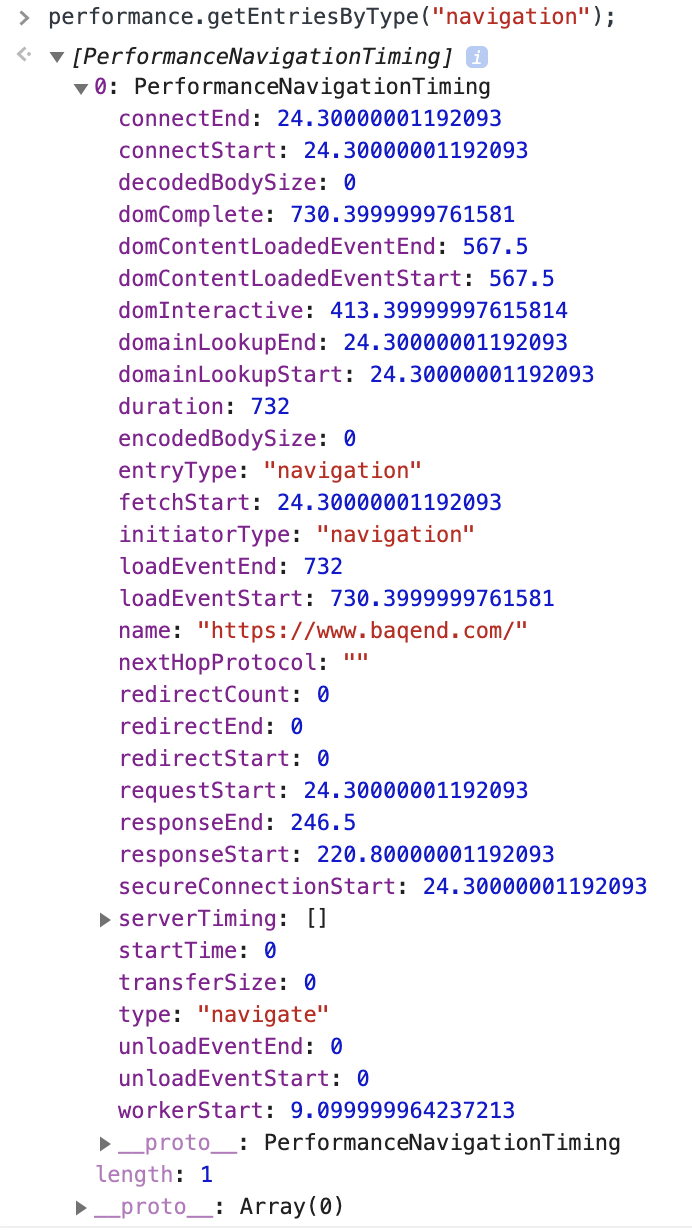
\includegraphics[width=0.4\textwidth]{navigation_console.png}
\caption{Navigation Timings, taken from Chrome's console log}
\label{figure:navigation_console}
\end{center}
\end{figure}


%TODO add this ?

% 2013 Grigorik
%- The real benefit of Navigation Timing is that it exposes a lot of previously inaccessible data, such as DNS and TCP connect times, with high precision (microsecond timestamps), via a standardized performance.timing object in each browser.
%- Hence, the data gathering process is very simple: load the page, grab the timing object from the user’s browser, and beacon it back to your analytics servers!
%- By capturing this data, we can observe real-world performance of our applications as seen by real users, on real hardware, and across a wide variety of different networks.

% 2013 Meenan
%- The largest benefit of navigation timing is that it exposes a lot of timings that lead up to the HTML loading --> This is this famous image
%- In addition to providing a good start time, it exposes information about any redirects, DNS lookup times, time to connect to the server, and how long it takes the Web server to respond to the request, for every user and for every page the user visits
%- The measurement points are exposed to the DOM (Document Object Model) through the performance object and make it trivial to calculate load times (or arbitrary intervals, really) from JavaScript.

% https://developer.mozilla.org/en-US/docs/Web/API/PerformanceNavigationTiming
%PerformanceNavigationTiming Interface: 
%- extends PerformanceEntry Interface from performance timeline. see attributes section for details
%- extends PerformanceResourceTiming Interface from resource timing

% ---------------------------------------------

\paragraph{Resource Timing} % korrigiert

% [Introduction]

There are two versions of Resource Timing.
A Candidate Recommendation, Resource Timing Level 1, from March 2017 \cite{2017W3CResourceTimingLevel1},
and Resource Timing Level 2, the current Working Draft \cite{2021W3CResourceTimingLevel2}.

Navigation Timing outputs timing information for the main document, while Resource Timing outputs timing information for all other resources that the main document requests, and also for resources that request other resources.
Other resources can be CSS, JS, other HTML documents, images and so on  \cite{2021W3CResourceTimingLevel2}.

The timestamps displayed by Resource Timing are mainly network-related time values (see table \ref{table:navigation_resource_attributes}).
For example, the time it takes to download a particular resource.

% [PerformanceResourceTiming Interface]

The Resource Timing values are provided by the PerformanceResourceTiming interface and can be retrieved in the browser via $window.performance.getEntriesByType("resource")$.

% https://w3c.github.io/perf-timing-primer/
%- The PerformanceResourceTiming interface extends the PerformanceEntry interface in the Performance Timeline
%- Each of these timestamps is in microseconds, which are provided by the window.performance.now() method in the High Resolution Time specification.

% [Navigation and Resource Timing]

Navigation and Resource Timing go hand in hand.
With Navigation and Resource Timing, all relevant timing information is available for all resources on the site.
The waterfall diagram (see Section X.) is an illustrative example of a visualization of the attributes provided by both specifications.
The attributes provided by Navigation and Resource Timing are discussed in more detail below.


% ---------------------------------------------

\paragraph{Navigation and Resource Timing Attributes} % korrigiert

All time values or attributes relevant to the navigation process and captured by Navigation and Resource Timing Level 2 are listed in Table \ref{table:navigation_resource_attributes} and Figure \ref{figure:navigation_resource_timestamps}.
The black coloured timestamps associated with the blue boxes in Figure \ref{figure:navigation_resource_timestamps} are captured by Navigation Timing.
The yellow coloured timestamps are captured by Resource Timing.
All attributes can be accessed in the browser via $performance.getEntriesByType("navigation")$.
Figure \ref{figure:navigation_resource_timestamps} does not contain all defined and available values from the specification definitions, but only those visible within the navigation process.
For documents with different origins, the attributes in parentheses may not be available \cite{2021W3CNavigationTimingLevel2}.


\begin{figure}[h!]
\begin{center}
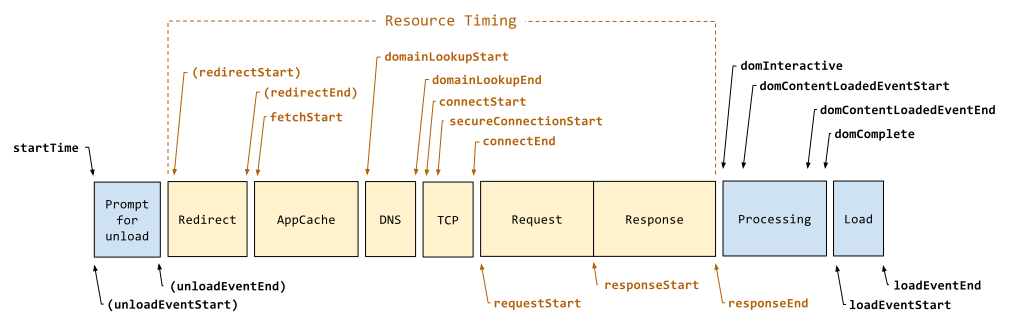
\includegraphics[width=1\textwidth]{timestamp_diagram.png}
\caption[Timestamps from Navigation and Resource Timing]{Timestamps from Navigation and Resource Timing, taken from \cite{2021W3CNavigationTimingLevel2}}
\label{figure:navigation_resource_timestamps}
\end{center}
\end{figure}


Table \ref{table:navigation_resource_attributes} provides a brief explanation for each timestamp.
The definitions are taken directly from the W3C specifications or MDN Web Docs, unless otherwise noted.
These timestamps are used to calculate performance metrics, as described in the next section.


\begin{center}
	\small
	\begin{longtable}{ | p{0.3\linewidth} | p{0.6\linewidth} | }
	\hline
	\multicolumn{2}{|c|}{ \cellcolor{lightgrey} Navigation Timings Level 2} \\
	\hline
	startTime (= navigationStart) & Start time of the navigation process. Is set to 0. Navigation Timing Level 1 exposes "navigationStart" which is set to the "time immediately after the user agent finishes prompting to unload the previous document."\footnote{\url{https://www.w3.org/TR/navigation-timing/)} [15.07.2021]} Since some metric calculations are still based on navigationStart (see below), it is mentioned here. \\
	\hline
	unloadEventStart & Set to 0 if there is no previous document. Otherwise, the value is set to the time when the event to unload the previous document is triggered by the user agent. \\
	\hline
	unloadEventEnd & Set to 0 if there is no previous document. Otherwise, the value is set to the time when the event to unload the previous documents ends. \\
	\hline
	domInteractive & Time value equal to the time immediately before the user agent sets the current document readiness of the current document to "interactive". \\
	\hline
	domContentLoadedEventStart & Time value equal to the time immediately before the user agent fires the DOMContentLoaded event at the current document. \\
	\hline
	domContentLoadedEventEnd & Time value equal to the time immediately after the current document's DOMContentLoaded event completes.  \\
	\hline
	domComplete & Time value equal to the time immediately before the user agent sets the current document readiness of the current document to "complete". \\
	\hline
	loadEventStart & Time value equal to the time immediately before the load event of the current document is fired. Returns 0 if the event was not triggered. \\
	\hline
	loadEventEnd & Time value equal to the time when the load event of the current document is completed.  Returns 0 if event has not been fired or is not completed. \\

	\hline
	\multicolumn{2}{|c|}{ \cellcolor{lightgrey} Resource Timings Level 2} \\
	\hline
	redirectStart & Start time of the fetch which initiates the redirect. \\
	\hline
	redirectEnd & Marks timestamp which occurs immediately after receiving the last byte of the response of the last redirect. \\
	\hline
	fetchStart & Marks when the browser starts to fetch a resource. Does not mark when the browser makes a network request for a resource, but rather when it begins checking caches to see if a network request is even necessary.  \\ % cite https://developers.google.com/web/fundamentals/performance/navigation-and-resource-timing
	% Represents a timestamp immediately before the browser starts to fetch the resource. \\
	\hline
	domainLookupStart & Returns the timestamp immediately before the browser starts the domain name lookup for the resource. \\
	\hline
	domainLookupEnd & Returns the timestamp immediately after the browser finishes the domain name lookup for the resource. \\
	\hline
	connectStart & Returns the timestamp immediately before the user agent starts establishing the connection to the server to retrieve the resource. \\
	\hline
	secureConnectionStart & Returns a timestamp immediately before the browser starts the handshake process to secure the current connection.  \\
	\hline
	connectEnd & Returns the timestamp immediately after the browser finishes establishing the connection to the server to retrieve the resource.  \\
	\hline
	requestStart & When the browser issues the network request.  \\% cite https://developers.google.com/web/fundamentals/performance/navigation-and-resource-timing
	% Returns a timestamp of the time immediately before the browser starts requesting the resource from the server, cache, or local resource. \\
	\hline
	responseStart & Returns a timestamp immediately after the browser receives the first byte of the response from the server, cache, or local resource. \\
	\hline
	responseEnd & Returns a timestamp immediately after the browser receives the last byte of the resource or immediately before the transport connection is closed, whichever comes first. \\
	\hline
	\caption[Navigation and Resource Timing Level 2 Attributes]{Navigation and Resource Timing Level 2 Attributes, taken from \cite{2021W3CNavigationTimingLevel2}, \cite{2021W3CResourceTimingLevel2}} % needs to go inside longtable environment
	\label{table:navigation_resource_attributes}
	\end{longtable}
\end{center}


The document states and events mentioned above, such as DOMContentLoaded, and their triggering by the user agent are defined in the HTML standard.


% add values from other interfaces such as duration ?
%from PerformanceEntry Interface:
%name
%entryType
%startTime
%duration
% add exposed as DOMHighResTimeStamp ?


%TODO add this when there is time...

% [Implementation Example Chrome]

% lets see how chromium is capturing domContentLoaded

% more infos here (probably level 1)
% https://community.akamai.com/customers/s/article/Using-Navigation-Timing-APIs-to-understand-your-webpage?language=en_US

% https://developers.google.com/web/fundamentals/performance/navigation-and-resource-timing
% Requests and responses:
%- fetchStart marks when the browser starts to fetch a resource. This is distinct from a request in that it doesn't mark when the browser makes a network request for a resource, but rather when it begins checking caches (e.g., HTTP and service worker caches) to see if a network request is even necessary.
%- workerStart marks when a request is being fetched from a service worker within a fetch event handler (if applicable). This will be always be 0 if a service worker isn't installed for the current page.


% ---------------------------------

\paragraph{Metrics calculated with Navigation and Resource Timing} % korrigiert

The attributes provided by Navigation and Resource Timing are used to compute common metrics for navigation timing.
Table \ref{table:navigation_timing_metrics} lists a selection of metrics for navigation timing and shows how they are derived from the attributes provided by Navigation and Resource Timing.
Figure \ref{figure:navigation_timing_metrics} provides a graphical overview of the metrics and the intervals they reflect.

As with web analytics metrics, there is no single source of truth or set of definitions for navigation timing metrics.
However, a review of the literature reveals a common set of navigation timing metrics.
Literature sources include the MDN Glossary\footnote{\url{https://developer.mozilla.org/en-US/docs/Glossary} [13.08.2021]},
Google developer guides \cite{2020Wagner},
blog posts by other performance specialists \cite{2020GTmetrix},
research papers (\cite{2013Wang}, \cite{2018Netravali}, \cite{2019Enghardt})
or the documentation of common RUM tools.\footnote{\url{https://github.com/akamai/boomerang/blob/master/doc/methodology.md} [13.08.2021]}

The sources mentioned above sometimes explain the idea of metrics in a rather informal way.
How exactly the metrics are implemented and calculated, e.g. which navigation timing attributes are used, is not always clear and is the responsibility of the RUM tool providers and can only be checked directly in the source code.
Due to the lack of standardization and definition of the metrics, it is therefore possible that different calculations are used for the same metric.

% add this ?
%- navigationStart is not in level 2
%- navigationStart is the same as startTime in level 2
%- Difference is that navigationStart is a EPOCH time stamp. The timings have to be calculated as differences to this timestamp
%- navigationStart just starts with 0, which makes all the other timestamps easier to read
%- many still use level 1 and navigationStart

% sort those metrics according to their occurance ? Which occurace ?

\begin{center}
	\small
	\begin{longtable}{ | p{0.3\linewidth} | p{0.6\linewidth} | }
	\hline
	Time to First Byte (TTFB)
	& $[responseStart - navigationStart]$ \\
	& Indicates when the user agent received the first byte of the websites data. \\
	& "Time it takes between the start of the request and the start of the response" \cite{2021MDNTTFB}.  \\
	% add more here ?
	
	\hline
	Page Load Time (PLT)
	& $[loadEventStart - navigationStart]$ \\
	& The MDN Docs define PLT as the "time it takes for a page to load" and it is calculated as stated in the square brackets \cite{2021MDNPLT}.  \\
	& Across multiple authors, PLT is defined as the time from navigation start until the load event\footnote{\url{https://developer.mozilla.org/en-US/docs/Web/API/Window/load_event} [16.07.2021]} has been fired.
	The load event is fired when the main document and its associated resources have been loaded. \\
	& Grigorik notes that PLT "has been the de facto metric of the web performance world" \cite{2013Grigorik}, but is inaccurate today due to the shift from static websites to dynamic web applications that load resources differently (see also \cite{2018Netravali}, \cite{2013Souders}). \\
			
		% more here ?
		% Akamai defines PLT similarly as the elapsed time from navigation start until the "page is completely available for the user to interact with", using also loadEventStart as the point when loading has finished.
		% cite https://github.com/akamai/boomerang/blob/master/doc/methodology.md, https://community.akamai.com/customers/s/article/Using-Navigation-Timing-APIs-to-understand-your-webpage?language=en_US
		%Wang et al define PLT as the "time between when the page is requested and when the DOMLoad event is fired", where the DOMLoad event is the load event.\footnote{\url{https://developer.mozilla.org/en-US/docs/Web/API/Window/load_event} [16.07.2021]}      % cite 2013 Wang
		% 2019 Enghardt
	
	\hline
	DNS Lookup Time
	& $[domainLookupEnd - domainLookupStart]$ \\
	& Time it takes for a DNS lookup \cite{2021MDNNavigationAndResourceTimings}, \cite{2020Wagner}. \\
	
	\hline
	TCP Handshake % / Server Connect Time ?
	& $[connectEnd - connectStart]$ \\
	& Time it takes for the TCP handshake \cite{2021MDNNavigationAndResourceTimings}. \\
% https://community.akamai.com/customers/s/article/Using-Navigation-Timing-APIs-to-understand-your-webpage?language=en_US
% https://developer.mozilla.org/en-US/docs/Web/Performance/Understanding_latency
	% Also called Connection Time.  % https://developers.google.com/web/fundamentals/performance/navigation-and-resource-timing

	\hline
	TLS Handshake Time
	& Time it takes to secure connection with TLS.  \\
	& MDN Docs defines TLS time with $[requestStart - secureConnectionStart]$ \cite{2021MDNNavigationAndResourceTimings}. \\
	& Google defines TLS Time as $[connectEnd - secureConnectionStart]$ \cite{2020Wagner}. \\

	\hline
	Request Time, 
	& $[responseStart - requestStart]$ \\ 
	Server Response Time & How long it takes for the request \cite{2021MDNNavigationAndResourceTimings}. \\
	& Also called Server Response Time by Akamai \cite{2018Akamai}. \\
	
	\hline
	DOM Content Loaded
	& MDN defines this metric as the interval between the start and end points of the DomContentLoaded event\footnote{\url{https://developer.mozilla.org/en-US/docs/Web/API/Window/DOMContentLoaded_event} [13.08.2021]} $[domContentLoadedEventEnd - domContentLoadedEventStart]$ \cite{2021MDNNavigationAndResourceTimings}. \\
	& Akamai defines it as the time from the start of navigation to the end of the DOMContentLoaded event: $[domContentLoadedEventEnd - navigationStart]$ \cite{2018Akamai}. \\
	& Google defines the metric similarly to Akamai, but uses the start point instead of the end point of the event for the calculation (see section \ref{subsubsection:ga_metrics}):
$[domContentLoadedEventStart - navigationStart]$. \\

	\hline
	Page Download Time,
	& $[responseEnd - responseStart]$ \\
	Receiving Time,  & How long it takes to download the page. \\
	Transfer Time & Also called Transfer time by Akamai \cite{2018Akamai} or Receiving Time by MDN \cite{2021MDNLatency}. \\

	\hline
	Latency
	& $[responseStart - fetchStart]$ \\ 
	& Latency is defined as the elapsed time from when the browser requests the resource until the first byte from it is received (\cite{2018Akamai}, \cite{2021MDNLatency}). \\

	\hline
	DOM Interactive
	& $[domInteractive - navigationStart]$ \\
	& When the "browser has completed parsing the entire HTML and constructed the DOM" \cite{2018Akamai}. \\

	
%TODO add this? maybe check again after WPT done
%	\hline
%	DOM Complete &
%	\begin{itemize}[label={}, noitemsep,nolistsep, leftmargin=0cm]
%		\item 
%		\item 
%	\end{itemize} \\	

%	\hline
%	Redirect &
%	\begin{itemize}[label={}, noitemsep,nolistsep, leftmargin=0cm]
%		\item 
% https://developers.google.com/web/fundamentals/performance/navigation-and-resource-timing
% redirectStart and redirectEnd 
%	\end{itemize} \\

	\hline
	\caption{Navigation Timing Metrics} % needs to go inside longtable environment
	\label{table:navigation_timing_metrics}
	\end{longtable}
\end{center}


% add this to PLT ? as it is the same...
% window.onload:
% https://community.akamai.com/customers/s/article/Using-Navigation-Timing-APIs-to-understand-your-webpage?language=en_US
% Onload = loadEventEnd - loadEventStart -> not the same as PLT
% https://www.stevesouders.com/blog/2013/05/13/moving-beyond-window-onload/
% when window.onload() is fired

% https://speedcurve.com/blog/rendering-metrics/
% when window.onload() is fired

% add this ?
% DOM Processing to Interactive
% https://community.akamai.com/customers/s/article/Using-Navigation-Timing-APIs-to-understand-your-webpage?language=en_US

% DOM Interactive to Complete
% https://community.akamai.com/customers/s/article/Using-Navigation-Timing-APIs-to-understand-your-webpage?language=en_US

%Load Event Duration
% https://developer.mozilla.org/en-US/docs/Web/Performance/Navigation_and_resource_timings#load_event_duration
%load = timing.loadEventEnd - timing.loadEventStart 


% Duration
% https://developer.mozilla.org/en-US/docs/Web/Performance/Navigation_and_resource_timings#duration
% duration = PerformanceNavigationTiming.loadEventEnd - PerformanceEntry.startTime
% -> duration from performanceentry interface is from loadEventStart - start Time

% Loading
% https://developers.google.com/web/fundamentals/performance/navigation-and-resource-timing
%- loadEventStart and loadEventEnd

% Document processing
% https://developers.google.com/web/fundamentals/performance/navigation-and-resource-timing
%- domInteractive, domContentLoadedEventStart, domContentLoadedEventEnd, and domComplete

% Unloading
% https://developers.google.com/web/fundamentals/performance/navigation-and-resource-timing
%Document unloading:
%- unloadEventStart and unloadEventEnd 

% Sizes
% https://developers.google.com/web/fundamentals/performance/navigation-and-resource-timing
% Document and resource size:
%- transferSize is the total size of the resource including HTTP headers.
%- encodedBodySize is the compressed size of the resource excluding HTTP headers.
%- decodedBodySize is the decompressed size of the resource (again, excluding HTTP headers).


\begin{figure}[h!]
\begin{center}
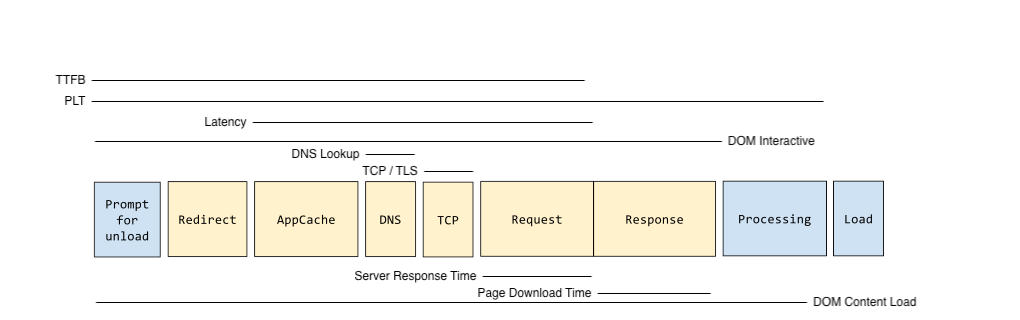
\includegraphics[width=1\textwidth]{nav_metrics.png}
\caption{Navigation Timing Metrics, graphical representation}
\label{figure:navigation_timing_metrics}
\end{center}
\end{figure}
%TODO make this nicer, e.g. use same font as text for labels


Apart from Navigation and Resource Timing, the Web Performance Working Group also maintains other performance-related specifications.
Some of these are briefly discussed below.

% ------------------------------------------------

\paragraph{User Timing} % korrigiert

User Timing Level 2 is a February 2019 Recommendation and User Timing Level 3 is the current Working Draft.
User Timing provides methods for creating custom, specific, and unique high-resolution timestamps, querying them, and calculating intervals and elapsed time between these created timestamps \cite{2021W3CUserTiming}.
User Timing simplifies and facilitates the use of Custom Metrics (see section \ref{subsection:custom_metrics}).

% https://www.w3.org/TR/user-timing-3/
%- PerformanceMark and PerformanceMeasure interfaces

% Measuring Real User Performance in the Browser https://www.youtube.com/watch?v=yrWLi524YLM&ab_channel=NicJansma
%-> Puts data in Performance Timeline / DevTools

% -------------------

\paragraph{Performance Timeline} % korrigiert

Performance Timeline is the December 2013 Recommendation \cite{2013W3CPerformanceTimeline} and Performance Timeline Level 2 is the current working draft \cite{2021W3CPerformanceTimelineLevel2}.

In short, the Performance Timeline defines an API and methods that make accessible all timing values captured by other specifications such as Navigation or Resource Timing.
The Performance Timeline defines an interface for capturing a variety of performance measurements. 
It can be used to retrieve Navigation Timings using $performance.getEntriesByType("navigation")$.

In addition, a PerformanceObserver interface is defined that can be used to monitor the Performance Timeline and notify when new measurements and recordings are available.

% add this ? is not so important...
% https://www.w3.org/TR/performance-timeline-2/
%- extends the High Resolution Time specification
%- providing methods to store and retrieve high resolution performance metric data.
%- Performance Timeline  defined by Navigation timing, resource timing, user timing and other interfaces
%- get Entries, by Type, by Name
%- Example entryType values defined by other specifications include: "mark" and "measure" [USER-TIMING-2], "navigation" [NAVIGATION-TIMING-2], "resource" [RESOURCE-TIMING-2], and "longtask"


% [Performance Entry]
	
% https://developer.mozilla.org/en-US/docs/Web/API/Performance_Timeline
%- PerformanceEntry interface encapsulates a single performance entry: a single data point or metric in the performance timeline

% https://developer.mozilla.org/en-US/docs/Web/API/PerformanceEntry
%- A performance entry can be directly created by making a performance mark or measure

%Always of type:
%- PerformanceMark
%- PerformanceMeasure
%- PerformanceFrameTiming
%- PerformanceNavigationTiming
%- PerformanceResourceTiming
%- PerformancePaintTiming

%Properties:
%- name
%- entryType
%- startTime
%- duration

% ----------------------------


\paragraph{Long Tasks} % korrigiert

The Long Tasks API 1 was released in September 2017 as a First Public Working Draft.
The goal of the API is to detect "long tasks", i.e. tasks that take the main thread longer than 50 ms.
Long tasks are critical to performance because they block other critical tasks such as user input \cite{2017W3CLongTasks}.

The Long Tasks API is used to calculate user-centric metrics (see section \ref{subsection:user_centric_performance_metrics}.

% add this here about metrics ?
%Long Tasks API is a basis to calculate metrics such as Time to Interactive (TTI) and Total Blocking Time (TBT). % https://web.dev/custom-metrics/#long-tasks-api
%TTI and TBT will be discussed below.

% https://github.com/WICG/time-to-interactive

% https://www.youtube.com/watch?v=6Ljq-Jn-EgU&ab_channel=GoogleChromeDevelopers
%- Long Tasks: Is it delightful? PerformanceObserver


% ----------------------------

\paragraph{Server Timing} % korrigiert

Server Timing is a Working Draft.
With specifications such as Navigation and Resource Timing, the user agent has access to a variety of different timings related to the navigation process.
Not visible or available are measurements and timings within server processing, such as database queries.
Server Timing solves this problem by allowing a server to transmit and communicate performance-related information to the user agent \cite{2021W3CServerTiming}.

% ----------------------------

\paragraph{Paint Timing} % korrigiert

Paint Timing 1 was published as a First Public Working Draft in September 2017.  
It specifies two "key moments" during the loading process: First Paint (FP) and First Contentful Paint (FCP).
Table \ref{table:paint_timing} provides explanations of the key moments as defined in the specification \cite{2017W3CPaintTiming}.

The metrics can be accessed directly in the browser via $performance.getEntriesByType("paint")$.
Therefore, FP and FCP can be captured in RUM.
Other visual metrics are mainly based on video analysis and require a synthetic monitoring facility as described in the next section.

\begin{table}[h]
	\small
	\centering
	\begin{tabular}{ | p{0.3\linewidth} | p{0.6\linewidth} | }
	\hline
	\textit{First Paint (FP)} & Marks the point when the browser renders anything that is visually different from what was on the screen prior to navigation \\ 
	\hline
	\textit{First Contentful Paint (FCP)} & The point when the browser renders the first bit of content from the DOM, which may be text, an image, SVG, or even a canvas element \\  
	\hline
	\end{tabular}
	\medskip
	\caption[Key Moments specified by Paint Timing]{Key Moments specified by Paint Timing, taken from \cite{2017W3CPaintTiming}}
	\label{table:paint_timing}
\end{table}

FP and FCP indicate when the user sees something other than the default white screen for the first time.
Whether the visual change is important or useful to the user is not considered by FP or FCP \cite{2013Meenan}.
Section \ref{subsection:user_centric_performance_metrics} discusses visual metrics that may be of importance to the user.

% add this ??
% As described below, FCP is part of Google's Web Vitals.
% For a more fine grained measurement, they enhance the default metric.

% add more here ?
% https://developer.mozilla.org/en-US/docs/Glossary/First_paint
% https://developer.mozilla.org/en-US/docs/Glossary/First_contentful_paint
% A user centric metric pendant is Start Render.
% FP and FCP are visual metrics from a browsers perspective, and not from a users perspective, as they are derived from  and not the actual pixels on the screen.

% ----------------------------

\paragraph{Web Incubator Community Group} % korrigiert

The Web Incubator Community Group (WICG) is a W3C Community Group and "provides a lightweight venue for proposing and discussing new web platform features."\footnote{\url{https://www.w3.org/community/groups/} [13.08.2021]}
The WICG is working on and proposing a number of possible web technologies and standards.\footnote{\url{https://wicg.io/} [24.07.2021]}
These specifications are unofficial drafts that have not been reviewed by the W3C, but may be included in the W3C Recommendations track in the future.
Four of the proposed "incubations" are mentioned here because they serve as the basis for some user-centric metrics, as described in Section \ref{subsubsection:core_web_vitals}.
Details on the specifications can be found on the corresponding pages:
\textit{Element Timing API}\footnote{\url{https://wicg.github.io/element-timing/} [24.07.2021]}, 
\textit{Event Timing API}\footnote{\url{https://wicg.github.io/event-timing/} [24.07.2021]},
\textit{Layout Instability API}\footnote{\url{https://wicg.github.io/layout-instability/} [24.07.2021]}, and
\textit{Largest Contentful Paint}.\footnote{\url{https://wicg.github.io/largest-contentful-paint/} [24.07.2021]}.

% https://web.dev/custom-metrics/
% Element Timing used for LCP
% Event Timing used for FID
%  Editors are from Google, close relation to Core Web Vitals
% Only available in Chromium

% ?? Network Information API (not official w3c) https://wicg.github.io/netinfo/

% ---------------------------------------------------------------------------------------------

\subsubsection{Navigation Timing Metrics Conclusion} % korrigiert

A variety of measurements and time intervals can be taken during the loading process of a website.
The W3C and the Performance Working Group maintain and define a set of specifications with the task of measuring performance and navigation timing data.
The attributes exposed by these specifications are used to calculate performance and navigation timing metrics.

Since the performance metrics are not officially defined by any authorized party or institution, their meaning may vary depending on the implementation.

Table \ref{table:apis_summary} provides an overview of all specifications discussed, at what maturity level they are available, and why they are important.


%The High Resolution Time recommendation enables exact, stable and reliable time measures.
%The Navigation and Resource Timing specifications expose all relevant time stamps on the document, or any resource respectively, loading process.
%The User Timing spec makes it possible for analysts and developers to mark and measure custom time stamps and expose them directly to the Performance Timeline.
%The Performance Timeline subsumes all exposed timing measures and is the go to place to fetch performance data.

%Or as Grigorik states it, "The combination of Navigation, Resource, and User timing APIs provides all the necessary tools to instrument and conduct real-user performance measurement for every web application" % cite 2013 Girgorik


\begin{table}[h]
	\small
	\centering
	\begin{tabular}{ | p{0.3\linewidth} | p{0.6\linewidth} | }
	\hline
	High Resolution Time
	& Level 2: REC November 2019 \\
	& Current WD \\
	& Provides accurate, stable and reliable time measurements. \\
	\hline
	Navigation Timing
	& Level 1: REC December 2012 \\
	& Level 2: Current WD \\
	& Exposes information about the navigation timing of the main document. \\
	\hline
	Resource Timing
	& Level 1: CR March 2017 \\
	& Level 2: Current WD \\
	& Exposes timing information of requested resources and the resources they requested. \\
	\hline
	Navigation and Resource Timing
	& Used to calculated a variety of metrics. \\
	\hline
	User Timing
	& Level 2: REC February 2019 \\
	& Level 3: Current WD \\
	& Mark and measure custom timestamps. \\
	\hline
	Performance Timeline
	& REC December 2013 \\
	& Level 2: Current WD \\
	& Subsumes collected performance data from other specifications. \\
	\hline
	Long Tasks
	& API 1: FPWD  September 2017 \\
	& Identifies tasks that occupy the main thread for more than 50ms. \\
	& Basis for TTI and TBT. \\
	\hline
	Server Timing
	& Current WD \\
	& Standard for transmitting performance-related data from the server to the client. \\
	\hline
	Paint Timing
	& FPWD September 2017 \\
	& Exposes the "key moments" First Paint and First Contentful Paint. \\
	\hline
	Element- and Event Timing API & WICG proposals (unoffical drafts), used for LCP, FID, CLS  \\
	Layout Instability API & \\ %TODO more ?
	Largest Contentful Paint & \\
	\hline
	\end{tabular}
	\medskip
	\caption{Summary of W3C and WICG Specifications}
	\label{table:apis_summary}
\end{table}


% [Transition]

Paint Timing is already moving in a direction that seeks to measure user-perceived performance not just by measuring elapsed time between navigation events, but rather by observing visual changes as the website loads.
Although navigation times can help identify any bottlenecks or other technical problems during the loading process, they do not reflect how the user actually perceives the performance of the website loading process.
Since users primarily consume websites with their eyes, visual indicators are relevant and critical.

In recent years, a variety of visual and user-centric performance metrics have emerged, some of which Google is promoting.
They are discussed in the next section.

% -----------------------------------------------------------------------
% -----------------------------------------------------------------------

\subsection{User-Centric Performance Metrics} % korrigiert
\label{subsection:user_centric_performance_metrics}

% [Introduction]

The Navigation Timings described in Section \ref{subsection:navigation_timing_metrics} are measured directly via a set of Web APIs and are accessible via the browser.
Metrics that deal with user-perceived performance focus mainly on visual changes to the website and therefore cannot be captured directly via Web APIs.

Perceived performance deals with how fast a website "feels" to a user.
As described earlier in Section X., different users perceive performance differently depending on factors such as gender, region, or stress level.
Perceived performance can differ from actual load times, and user-centric performance metrics are typically more difficult to measure than navigation times because visual analysis or video recordings are required to calculate the metrics \cite{2021MDNPerceivedPerformance}.

In Section \ref{subsubsection:visual_metrics}, I describe user-centric performance metrics that have become mainstream among performance monitoring vendors.
With Web Vitals, Google defines its own set of user-centric metrics and focuses on website performance.
They are discussed in Section \ref{subsubsection:web_vitals}.

% ------------------------

\subsubsection{Visual Metrics} % korrigiert
\label{subsubsection:visual_metrics}

The term "Visual Metrics" is not defined by any specification or web technology association and is used here to subsume metrics that rely on the visual part of the website.
Visual metrics are based on the video recording of the website loading process and use this recording for further analysis.
Therefore, they are best suited for synthetic monitoring.
Visual metrics focus mainly on how fast pixels are rendered into the viewport, the part of the screen visible to the user.

The three metrics described below appear frequently in synthetic monitoring tools and other web performance literature referenced in their respective sections.


% ------------------------

\paragraph{Start Render, Time to First Paint (TTFP)} % korrigiert

The Start Render time is the time when the browser made the first pixel on the screen visible to the user.
The Start Render time is calculated using video analytics instead of using browser APIs such as Paint Timing \cite{2019Schapira}.

Start Render is defined and exposed by a number of synthetic monitoring solutions such as SpeedCurve \cite{2021Souders} or WebPageTest (see section \ref{subsubsection:wpt_metrics}).

Netravali et al. \cite{2018Netravali} use the term Time to First Paint (TTFP) for the same metric,
while for Enghardt et al. \cite{2019Enghardt} TTFP is the same as FP measured within the browser and not by video analysis.

This example shows that the definitions of metrics are not clear and different authors use different definitions.


% ------------------------

\paragraph{Above the Fold Time (AFT)} % korrigiert

The above-the-fold area is the area of the website that is visible to the user without scrolling.
Above the Fold Time (AFT) is a non-standard metric that measures how long it takes the browser to render all the pixels in this above-the-fold area \cite{2019Enghardt}.
AFT measurement must take into account both visually dynamic areas of the website, where frequent pixel changes are expected, and static areas, where pixel and color changes are not expecte \cite{2018Netravali}.

AFT is measurable by synthetic monitoring and requires video recording and analysis \cite{2013Meenan}.

% ------------------------

\paragraph{Speed Index (SI)} % korrigiert

The Speed Index (SI) is a metric developed by the founders of WebPageTest that aims to express user experience in a single number \cite{2013Meenan}.

Like the AFT, the SI reflects the visual completeness of the website.
While the AFT only measures the time at which the viewport is fully rendered, the SI also takes into account the visual loading progress of the website and reflects "the average time at which visible parts of the page are displayed" \cite{2018Netravali}.
SI is not measured directly, but calculated and expressed in milliseconds \cite{2021GTmetrix}.

Like AFT, SI is reliable for static websites and unreliable for websites with dynamic and changing visual content \cite{2021Wingerath}.
The details of the SI calculation are covered in the official WebPageTest documentation.\footnote{\url{https://docs.webpagetest.org/metrics/speedindex/} [13.08.2021]}

% 2021 Meenan vimeo 38:50
% Measuring Real User Performance in the Browser
%- How much of the screen is visually available at different points of time
%- At what point of time is the page complete

% ------------------------

\subsubsection{Web Vitals} % korrigiert
\label{subsubsection:web_vitals}

% [Introduction]

With the Web Vitals initiative, Google is participating in the discussion about web performance metrics.
Their goal is to "provide unified guidance for quality signals that are essential to delivering a great user experience on the web" \cite{2020WaltonVitals}.
Unified guidance consists of Web Vitals, a set of performance metrics that focus on how users experience and perceive performance, as opposed to just navigation timings, as discussed in Section \ref{subsection:navigation_timing_metrics}.
Since performance is a factor in Google search rankings, Web Vitals automatically become important to website owners \cite{2019OsmaniGrigorik}.

% [Evolving]

The set and definitions of Web Vitals metrics are not set in stone, but are constantly evolving.
The definitions, calculations, recommended thresholds, or even the metrics themselves may change over time, always adapted to the rapidly evolving technologies of the WWW and advances in web performance \cite{2020WaltonVitals}.
While Web Vitals is currently primarily about web performance, other aspects of usability, such as security, privacy, or accessibility, will be included in the future \cite{2020SullivanMichal}.

% [Definition and Key Questions]

Web Vitals and their definitions are derived from a set of key questions (table \ref{table:web_vitals_key_questions}).
The key questions reflect what users ask (possibly unconsciously) while using a website. 
This user-centered framework serves as a guide for creating and defining Web Vitals metrics.
Unlike navigation timing metrics, Web Vitals focus on users and their perceptions, and each question is a perspective or facet of the user experience.
Web Vitals are "metrics relevant to users" \cite{2019WaltonUserCentric}.


\begin{table}[h]
	\small
	\centering
	\begin{tabular}{ p{0.3\linewidth} | p{0.6\linewidth} }
	\textit{Is it happening?} & Did the navigation start successfully? Has the server responded? \\
	\hline
	\textit{Is it useful?} & Has enough content rendered that users can engage with it? \\
	\hline
	\textit{Is it usable?} & Can users interact with the page, or is it busy? \\
	\hline
	\textit{Is it delightful?} & Are the interactions smooth and natural, free of lag and jank? \\
	\end{tabular}
	\medskip
	\caption[Key Questions for defining Web Vitals]{Key Questions for defining Web Vitals, taken from \cite{2019WaltonUserCentric}}
	\label{table:web_vitals_key_questions}
\end{table}


% [Types of Metrics]

In addition to the key questions, Google identifies different aspects or types of website performance (table \ref{table:web_vitals_types}).
Like the key questions, these types provide a guide and framework for organizing, classifying, and integrating Web Vitals \cite{2019WaltonUserCentric}.

%TODO add more here, some interpretation ?

\begin{table}[h]
	\small
	\centering
	\begin{tabular}{ p{0.3\linewidth} | p{0.6\linewidth} }
	\textit{Perceived load speed} & How quickly a page can load and render all of its visual elements to the screen. \\
	\hline
	\textit{Load responsiveness} & How quickly a page can load and execute any required JavaScript code in order for components to respond quickly to user interaction. \\
	\hline
	\textit{Runtime responsiveness} & After page load, how quickly can the page respond to user interaction. \\
	\hline
	\textit{Visual stability} & Do elements on the page shift in ways that users don't expect and potentially interfere with their interactions? \\
	\hline
	\textit{Smoothness} & Do transitions and animations render at a consistent frame rate and flow fluidly from one state to the next? \\
	\end{tabular}
	\medskip
	\caption[Types of Web Vitals Metrics]{Types of Web Vitals Metrics, taken from \cite{2019WaltonUserCentric}}
	\label{table:web_vitals_types}
\end{table}

% add RAIL model? https://web.dev/rail/

% [Measurement and Tools]

Web Vitals can be measured by synthetic monitoring or RUM \cite{2019WaltonUserCentric}.
For example, RUM data is available through CrUX\footnote{\url{https://developers.google.com/web/tools/chrome-user-experience-report} [22.07.2021]}, synthetic data is available through Lighthouse\footnote{\url{https://developers.google.com/web/tools/lighthouse} [22.07.2021]}.
A custom JS library is available and can be integrated into any website to capture Web Vitals.\footnote{\url{https://github.com/GoogleChrome/web-vitals} [22.07.2021]}

% PageSpeedInsigths ?

% [Outline]

In the following, I describe common Web Vitals metrics.
Section \ref{subsubsection:core_web_vitals} discusses the Core Web Vitals, the most important Web Vitals.

% ------------------------

\paragraph{First Contentful Paint} % korrigiert

First Contentful Paint (FCP) deals with question \textit{Is it happening?} and is classified as type \textit{Perceived load speed}.
This is the same FCP as used by Paint Timing (see Section \ref{subsubsection:w3c_performance_specifications}), and "marks the first point in the page load timeline where the user can see anything on the screen" \cite{2019WaltonFCP}.

Google extends the Paint Timing specification with respect to FCP by only considering pages that are in the foreground all the time, by measuring FCP even when the page has been loaded from cache, and by exposing FCP for all frames, including cross-origin iframes.
Implementation details can be found in the web-vitals library.\footnote{\url{https://github.com/GoogleChrome/web-vitals/blob/main/src/getFCP.ts} [22.07.2021]}

FCP is measured in seconds and can be retrieved in synthetic and real-user monitoring \cite{2019WaltonFCP}.

% ------------------------

\paragraph{First Meaningful Paint} % korrigiert

First Meaningful Paint (FMP) is "the paint after which the biggest above-the-fold layout change has happened and web fonts have loaded" \cite{2021MDNFMP}.

Google states that FMP is no longer used due to "inconsistent results" and the inability to measure it in all web browsers \cite{2019GoogleFMP}.
FMP's successor, Largest Contentful Paint, is discussed below.
The replacement of FMP nicely illustrates the evolution of Web Vitals.

% https://medium.baqend.com/mobile-site-speed-measurement-best-practices-ff4a3f91b003
%The First Meaningful Paint is another user-centric metric and represents the point in time at which the largest visual change takes place; the underlying assumption here obviously is that the biggest visual change is relevant to the user, for example because a hero image or a navigation bar appear


% ------------------------

\paragraph{Time to Interactive and First CPU Idle} % korrigiert

% [Explanation]

Time to Interactive (TTI) is an indicator for \textit{Load responsiveness} and gives insights into the question \textit{Is it usable?}
TTI measures the "time from when the page starts loading to when its main sub-resources have loaded and it is capable of reliably responding to user input quickly" \cite{2019WaltonTTI}.
Previously, TTI was referred to as \textit{Time to Consistently Interactive} \cite{2017GoogleInteractive}.

Other metrics and definitions are needed to calculate TTI:
FCP as a starting point and a "quiet window", i.e. a time interval in which no long tasks (as defined by the API for long tasks, see section \ref{subsubsection:w3c_performance_specifications}) and no more than two in-flight GET requests occur.
% explain in-flight ? https://github.com/WPO-Foundation/webpagetest/blob/master/docs/Metrics/TimeToInteractive.md
The TTI is then the "end time of the last long task before the quiet window".
The time interval for the quiet window is set to 5 seconds, and the starting point for the search for TTI is FCP.
% Hence, TTI is not a real time metric, as at least 5 seconds need to elapse first.
To summarize, "TTI measures how long it takes a page to become fully interactive" \cite{2021GoogleTTI}.

Ideally, the time between FCP and TTI, i.e. when the content is visible but the website is not interactive, is short.
The TTI can be measured by synthetic monitoring and also by RUM.
The latter is not recommended because user interaction can influence the TTI, leading to unreliable results.

% [First CPU Idle]

\textit{First CPU Idle} is a metric closely related to TTI.
Previously, First CPU Idle was called \textit{First Interactive} \cite{2017GoogleInteractive}.
First CPU Idle indicates when the website is minimally interactive, as opposed to the TTI, which indicates when the website is fully interactive.
Google deprecated First CPU Idle, as "the difference [to TTI] isn't significant enough to justify maintaining two similar metrics" \cite{2019GoogleFirstCPUIdle}.

% ------------------------

\paragraph{Total Blocking Time} % korrigiert

% [Explanation] 

Total Blocking Time (TBT) captures the aspect of \textit{Load responsiveness} and provides clues to the question \textit{Is it happening?}.
By definition, TBT measures "the total amount of time between First Contentful Paint (FCP) and Time to Interactive (TTI) where the main thread was blocked for long enough to prevent input responsiveness" \cite{2020WaltonTBT}.
The starting point of the measurement is the point of the FCP, since user input is unlikely to occur before the user interface is rendered.
The end point of the measurement is the point of the TTI.

Blocking the main thread is characterized by long tasks as defined in the Long Task API (see Section \ref{subsubsection:w3c_performance_specifications}).
If the user interacts with the website while a long task is running, the browser cannot respond to the user until it finishes processing the long task.
Therefore, the user must wait.
The blocking time of a long task is the total time of the task minus the defined long task time of 50 ms.
For example, a long task of $180ms$ has a blocking time of $180ms - 50ms = 130ms$.
The sum of all these times, between FCP and TTI, is the TBT.

% [Link to TTI]

For some use cases, TBT can adjust and correct the TTI if the TTI does not realistically reflect the available interactivity:
Since the TTI is fixed around a 5-second time window, the TTI is likely to be the same for (A) three long tasks of 51 ms spread over 10 seconds, and (B) one 10-second task.
(A) is likely to be more interactive because the main thread can respond to user input between the three long tasks.
In (B), on the other hand, the main thread is blocked and user interactivity is prohibited.
For such use cases, TBT is a good indicator:
For (A), TBT is 3ms and for (B) it is 9950 ms.
The lower the TBT value, the better the interactivity and user experience.

As with TTI, Google recommends measuring TBT by synthetic monitoring and not by RUM, since user input can influence and interfere with the measurement results. \\

% [Transition]

Among the Web Vitals, there are three metrics that are most important.
The \textit{Core Web Vitals} will be discussed next.


% ----------------------------------------

\subsubsection{Core Web Vitals} % korrigiert
\label{subsubsection:core_web_vitals}

Within Web Vitals, there is a group of metrics that are most important:
"Core Web Vitals are the subset of Web Vitals that apply to all web pages, should be measured by all site owners, and will be surfaced across all Google tools" \cite{2020WaltonVitals}.
The Core Web Vitals are structured around the performance aspects \textit{Loading}, \textit{Interactivity}, and \textit{Visual Stability}.
Each of three Core Web Vitals reflects one of those aspects (table \ref{table:core_web_vitals}).

The Core Web Vitals are relevant for all types of websites and can be measured with RUM.
In contrast to the general development of the Web Vitals, the Core Web Vitals are relatively stable in terms of definition and recommended benchmarks \cite{2020WaltonVitals}.

Core Web Vitals are captured by common Google performance evaluation tools such as CrUX or PageSpeed Insights,\footnote{\url{https://developers.google.com/speed/pagespeed/insights/} [23.07.2021]}
and are also made available via the web-vitals library.\footnote{\url{https://github.com/GoogleChrome/web-vitals} [23.07.2021]}

\begin{table}[h]
	\small
	\centering
	\begin{tabular}{  p{0.3\linewidth} | p{0.6\linewidth} }
	\textit{Largest Contentful Paint (LCP)} & Measures loading performance.  \\
	\hline
	\textit{First Input Delay (FID)} & Measures interactivity. \\
	\hline
	\textit{Cumulative Layout Shift (CLS)} & Measures visual stability.  \\
	\end{tabular}
	\medskip
	\caption{Core Web Vitals}
	\label{table:core_web_vitals}
\end{table}

The three Core Web Vitals LCP, FID and CLS are discussed in more detail below.

% --------------------

\paragraph{Largest Contentful Paint (LCP)} % korrigiert

% [Explanation]

Largest Contentful Paint (LCP) looks at \textit{Perceived load speed} and answers the question \textit{Is it useful?}.
While other metrics such as FCP or SI indicate when the first color is rendered on the screen or how fast the rendering process is, LCP is a metric used to report when the main content is visible to the user, where the main content is defined as the largest element.
In short, LCP is "the render time of the largest image or text block visible within the viewport, relative to when the page first started loading" \cite{2020WaltonLCP}.

To find the largest element, for example, images, videos or block elements with text are considered.
The size of an element is defined as only the area that is visible to the user.
LCP candidates can change during the loading process and are reported until the user interacts with the page.

LCP is defined and disclosed by the WICG specification \textit{Largest Contentful Paint}.
As with other metrics that rely on W3C specifications and APIs such as FCP, Google makes minor adjustments and, for example, only considers pages that were loaded in the foreground.
Implementation details are available in the web-vitals library.\footnote{\url{https://github.com/GoogleChrome/web-vitals/blob/main/src/getLCP.ts} [22.07.2021]}
The advantage over other visual metrics such as SI is that LCP is retrievable not only in synthetic monitoring but also in RUM \cite{2020WaltonLCP}.

% [Issues]

Although the Core Web Vitals are intentionally kept fairly stable in their definitions, Google's performance measurement initiative is still an evolutionary process that is not yet complete:
For example, a change in Google Chrome's LCP measurement changed LCP scores by 20\% \cite{2021Gessert}.
Changes and improvements to the definition and implementation of Web Vitals are not uncommon, as can be seen from the Chromium Web Vitals changelog.\footnote{\url{https://chromium.googlesource.com/chromium/src/+/refs/heads/main/docs/speed/metrics_changelog/README.md} [24.07.2021]}

% maybe largest element is not most important one... use custom metrics.

% --------------------------

\paragraph{First Input Delay (FID)} % korrigiert

% [Explanation]

First Input Delay (FID) has to do with \textit{Load responsiveness} and answers the question \textit{Is it usable?}.
FID provides information about website responsiveness and interactivity and measures "the time from when a user first interacts with a page (i.e. when they click a link, tap on a button, or use a custom, JavaScript-powered control) to the time when the browser is actually able to begin processing event handlers in response to that interaction" \cite{2020WaltonFID}.
Continuous events such as scrolling or zooming are not counted as initial inputs.

FID is about the time it takes for the browser to process user input.
This time depends on the tasks of the main thread:
If the main thread is busy while the user is interacting with the page, the browser must wait until the main thread is idle and can respond.
In technical terms, "FID measures the delta between when an input event is received and when the main thread is next idle" \cite{2020WaltonFID}.
By this definition, FID is measured even if no event listener is registered to process the user input, since only the main thread and its idle state are included in the equation.

FID only considers \textit{first input} because first input, and thus first impression, is critical and likely to be triggered during website loading, where interactivity and performance issues are more common than when the website is already loaded \cite{2020WaltonFID}.

% [RUM]

FID can only be measured in the field because it requires real user interaction.
Since FID depends on when a user interacts with the page, i.e., some users do not interact with the page at all, some interact when the main thread is busy, and others when the main thread is idle, it is important to analyse the distribution of reported FID values.
In synthetic monitoring, an alternative and proxy metric of FID is TBT, as it "correlates well with FID" \cite{2020WaltonFID}.

% [API]

FID is measurable with the WICG specification \textit{Event Timing API}.
As with other metrics that rely on W3C specifications and APIs such as FCP, Google makes minor adjustments and, for example, only considers pages that were loaded in the foreground.
Implementation details are available in the web-vitals library.\footnote{\url{https://github.com/GoogleChrome/web-vitals/blob/main/src/getFID.ts} [22.07.2021]}

% --------------------------

\paragraph{Cumulative Layout Shift (CLS)} % korrigiert

Cumulative Layout Shift (CLS) is about \textit{Visual stability} and answers the question \textit{Is it delightful?}.
CLS measures "unexpected movement of page content" \cite{2020WaltonCLS}.
\textit{Layout shift scores} are calculated for this purpose.
Layout shift scores reflect and evaluate the unexpected movement of visible elements between frames (\textit{layout shifts}).
Layout shift scores are calculated by other measures such as \textit{impact fraction} and \textit{distance fraction}, which evaluate the movement of visible elements.
The rather complex calculations are described in \cite{2020WaltonCLS}.
Finally, layout shifts over the lifetime of a page are summed (accumulated) and reported as CLS.
CLS is a score and not a value representing milliseconds.

CLS is based on the WICG specification \textit{Layout Instability API}.
As with other metrics that rely on W3C specifications and APIs such as FCP, Google makes minor adjustments to the specification, such as only considering pages that were loaded in the foreground.
Details about the CLS implementation are available in the web-vitals library.\footnote{\url{https://github.com/GoogleChrome/web-vitals/blob/main/src/getCLS.ts} [22.07.2021]}
CLS is retrievable by synthetic or real-user monitoring \cite{2020WaltonCLS}.

% [New CLS]

As observed with other metrics and Web Vitals, changes to the definitions of metrics or their implementation are not uncommon.
For CLS, the implementation changed in June 2021 \cite{2021Sullivan}.
This change shows once again that web performance metrics are rather fragile and still under development.

% https://blog.webpagetest.org/posts/understanding-the-new-cumulative-layout-shift/?utm_medium=email&_hsmi=121601471&_hsenc=p2ANqtz-9IsSdXActEE6lw4BrDZNa4eFqzQZjgabLHbq7aS-c2KkhqLGNtkIaGfQYD4VqZe9_6ZYFlTmlCgB87THSfsnVM1fl7NiixtrJqAsVO6DPUjeJIo6c&utm_content=121601471&utm_source=hs_email


% --------------------------

\paragraph{Core Web Vitals Thresholds} % korrigiert

For each of the Core Web Vitals, Google provides thresholds and recommended goals described as \textit{Good}, \textit{Needs Improvement}, and \textit{Poor}.
The rationale for these thresholds is briefly explained in this section.

Google considers values determined by researchers in the fields of Human-Computer Interaction and Human Perception for its threshold definitions.
Referenced studies are for example \cite{2004Galletta}, \cite{2000Hoxmeier}, and \cite{2005Oulasvirta}.

When research is not available, such as with CLS, a relatively new metric, Google relies on its own studies and assessments from the field.
The proposed thresholds are realistic enough to be met and achieved by normal websites.
The thresholds are therefore based on available data (e.g., from CrUX).
The best possible rating of "good," defined as "high-quality user experience", is defined as being exceeded by 10\% of all websites.
With new research, technology, and other improvements, the thresholds may be adjusted in the future \cite{2020McQuade}.

Figure X shows the threshold values for the three Core Web Vitals LCP, FID and CLS.
While LCP and FID are specified in milliseconds, CLS is a calculated value.
The exact rationale for the thresholds set for the Core Web Vitals can be found in \cite{2020McQuade}.

%TODO put them in one figure and use figure caption
%TODO always write: taken from url.... !!! for all figures
\begin{table}[h]
	\centering
	\begin{tabular}{ c c c }
	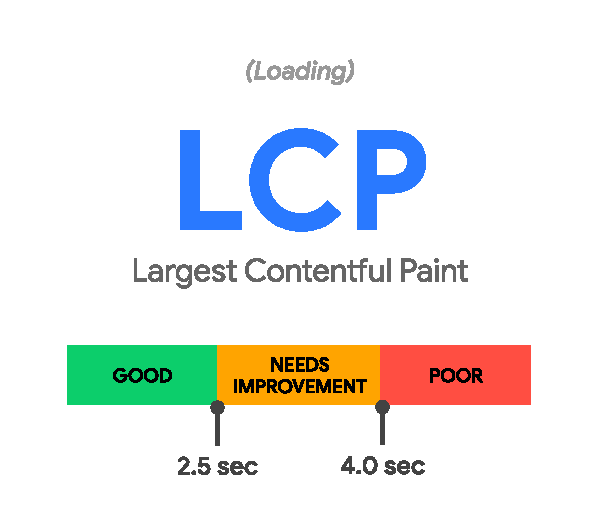
\includegraphics[width=0.3\textwidth]{lcp} &
	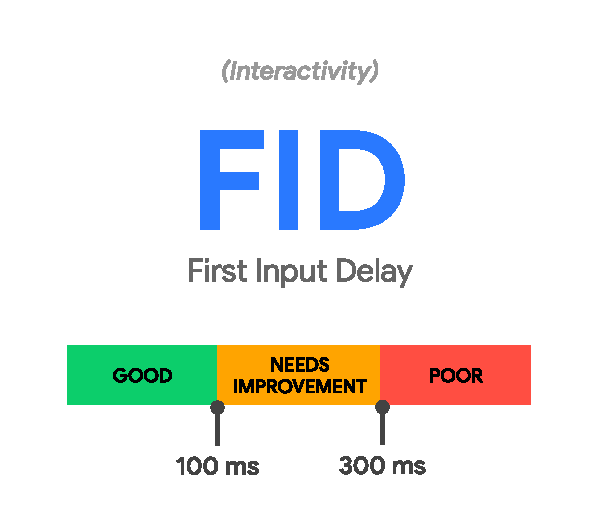
\includegraphics[width=0.3\textwidth]{fid} &
	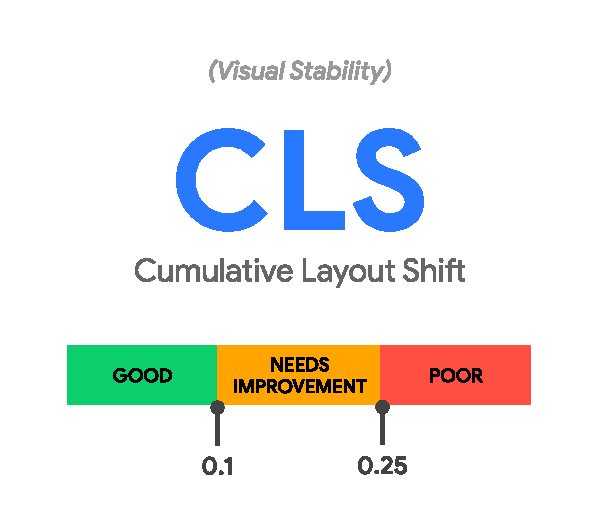
\includegraphics[width=0.3\textwidth]{cls} \\
	\end{tabular}
	\medskip
	\caption{Core Web Vitals Thresholds}
	\label{table:vitals_thresholds}
\end{table}

%\begin{figure}[h!]
%\begin{center}
%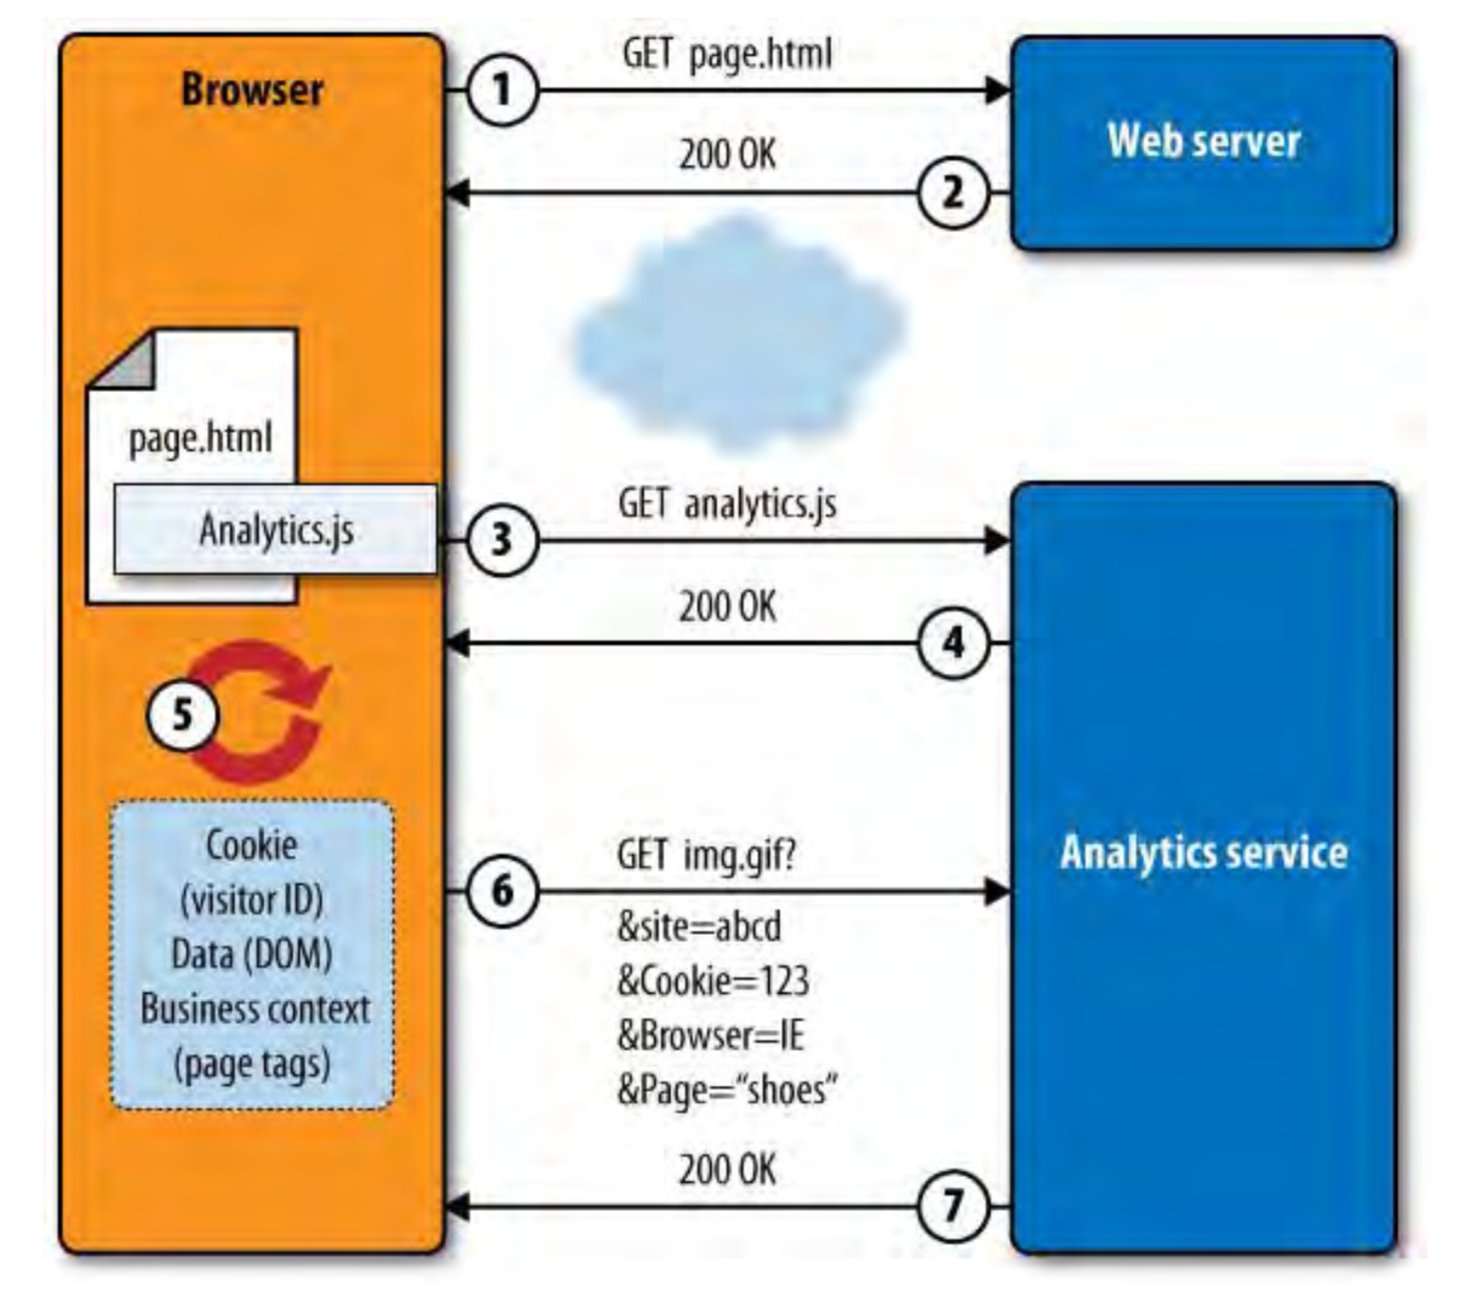
\includegraphics[width=0.5\textwidth]{page_tagging.png}
%\caption{Page Tagging}
%\label{img:page_tagging}
%\end{center}
%\end{figure}

% [75th percentile]

The classification of a website into one of the three classes is based on the 75th percentile value of all page views:
For a site to be classified as "good," at least 75\% of page views must exceed this threshold.
For example, if 25\% of the measured page views fall into the "poor" segment, the other two segments cannot reach the 75\%, so the page would be classified as "poor".
The reason for the 75th percentile is that it guarantees that a large portion of users are taken into account and that the value at the selected percentile is not too influenced by outliers.
The 75th percentile is a compromise between these two arguments: 3 out of 4 users experience the measured values, and 25 out of 100 samples can be outliers without affecting the result \cite{2020McQuade}.


% -----------------------------------------------------------------------

\paragraph{User-Centric Performance Metrics Conclusion} %  korrigiert

% [User-Centric vs Navigation Timings]

User-centric performance metrics aim to capture how users perceive, experience, and feel about performance.
This is in contrast to navigation timing metrics that rely only on in-browser timings that may have no meaning to the user.

% [Visual metrics]

Visual metrics such as Start Render or Speed Index are one approach to approximate and calculate how users perceive website performance by examining the pixels the browser renders into the viewport.
They rely on video recording and analysis and work best for synthetic monitoring.

% [Web Vitals and Core Web Vitals]

With Web Vitals, Google has introduced a set of user-centric performance metrics.
They are built and modelled around a set of guiding questions and performance types, as seen in table \ref{table:vitals_summary}.

Core Web Vitals are the three most important Web Vitals.
They reflect the loading performance (LCP), interactivity (FID), and visual stability (CLS) of the website.
Core Web Vitals can be measured using RUM.
Google provides a rating system for Core Web Vitals.
The thresholds for the ratings are derived from HIC and Human Perception research or derived directly from field data.

%TODO Also show which metrics are correlated, or which one replaced other ones ?

\begin{table}[h]
	\small
	\centering
	\begin{tabular}{ | l | l | l | l | l |}
	\hline
	\cellcolor{lightgrey} & Is it happening? & Is it useful? & Is it usable? & Is it delightful? \\
	\hline
	Perceived load speed & FCP & \underline{LCP} & & \\
	\hline
	Load responsiveness & & & TTI, TBT, \underline{FID} & \\
	\hline
	Runtime responsiveness & & & & \\
	\hline
	Visual stability & & & & \underline{CLS} \\
	\hline
	Smoothness & & & & \\
	\hline
	\end{tabular}
	\medskip
	\caption{Web Vitals and their position in the mental model. Core Web Vitals are underlined.}
	\label{table:vitals_summary}
\end{table}

As can be seen in table \ref{table:vitals_summary}, user-centric performance metrics do not yet exist for all questions and types, such as runtime responsiveness or smoothness.
Google indicates that new metrics are being introduced for some missing areas, but ideally custom metrics should be used in practice that capture the most important data for the business \cite{2019WaltonUserCentric}.
Custom metrics are discussed in the next section.

% Questions:
% Is it happening?
% XX FCP
% Is it useful?
% XX LCP
% Is it usable?
% XX TTI
% XX TBT
% XX FID
% Is it delightful?
% XX CLS
% Types:
% Perceived load speed
% XX FCP 
% XX LCP
% Load responsiveness
% XX TTI
% XX TBT
% XX FID
% Runtime responsiveness
% Visual stability
% XX CLS
% Smoothness


% -----------------------------------------------------------------------
% -----------------------------------------------------------------------

\subsection{Custom Metrics} % korrigiert
\label{subsection:custom_metrics}

% [Universal vs Custom]

The performance metrics described so far are relevant to gaining insight into page weight, such as how many requests it takes to build the website, to gaining an understanding of navigation timings, such as how long certain processes take in the CRP, and to gaining an understanding of user-perceived performance by calculating the Speed Index or measuring the time it takes to render the largest element.
These metrics are good for getting a general overview of the website's performance or comparing it to the competition, but they are not able to reflect the very unique and individual performance metrics tailored to the business.
Custom metrics are needed for this.

% https://web.dev/custom-metrics/
%- Universal metrics offer a good baseline, but in many cases you need to measure more than just these metrics in order to capture the full experience for your particular site.
%- Custom metrics allow you to measure aspects of your site's experience that may only apply to your site

% [References]

Almost all authors encourage and recommend the use of custom metrics:
Meenan notes that "nothing beats application-specific knowledge and measurements" \cite{2013Meenan}, and suggest, for example, a performance metric such as "Time to First Tweet" for Twitter \cite{2021MeenanKadlec}.
And Grigorik notes that "custom and application-specific metrics are the key to establishing a sound performance strategy" \cite{2013Grigorik}.

% 2013 Grigork
%- "there is no one single metric that holds true for every application, which means that we must carefully define custom metrics in each case"

% [Using APIs]

Custom JS code is required to measure custom metrics.
As described in Section \ref{subsubsection:w3c_performance_specifications}, several Web APIs are available to retrieve useful browser timings, i.e. paint events.
User Timing, in particular, is of particular interest for custom metrics, as it allows for the creation and retrieval of custom timestamps.
One disadvantage of custom metrics is that they are not comparable to any kind of benchmarks or competitors, since most likely no one else is measuring the exact same metric.


% -----------------------------------------------------------------------

\subsection{WebPageTest and Google Analytics Metrics} % korrigiert
\label{subsection:wpt_ga_metrics}

WebPageTest (WPT) and Google Analytics (GA) are common tools for synthetic monitoring and RUM, respectively (see section X).
Since they are used in the controlled experiment described in chapter X, the metrics they reveal are discussed in this section.


% ----------------------------------------------------------------

\subsubsection{WebPageTest Metrics} % korrigiert
\label{subsubsection:wpt_metrics}

WPT measures and delivers a variety of performance metrics.
First, I will briefly discuss how WPT categorizes its metrics.
Then, the most important metrics will be discussed, i.e., the metrics that are visible on the results pages after a test is run.
Next, the variety of website breakdowns offered by WPT is described.
Finally, two important performance analyses offered by WPT are briefly described: Waterfall charts and grades.


\paragraph{Metrics Categories} % korrigiert

According to the documentation\footnote{\url{https://docs.webpagetest.org/} [15.08.2021]}, there are two main categories for performance metrics: Page-Level metrics and Request-Level metrics.
Page-level metrics include technical and visual metrics, as described in Section X and Section X, as well as other site-related data such as page information, e.g. URL or DOM elements, or the state of the browser, e.g. its name or resolution.
Request-level metrics provide information about each individual request, such as the HTTP method used, DNS or TCP timings, and bytes received, to name a few.

Table X contains a summary of the categories.
Detailed descriptions of the categories and the metrics they contain can be found in the documentation.

\begin{table}[h]
	\small
	\centering
	\begin{tabular}{l | l}
	\hline
	Page-Level Metrics & Technical Page Metrics, Visual Metrics, \\
	& Interactivity Metrics, Javascript and CPU timings, \\
	& Page Information, Browser State \\
	\hline
	Request-Level Metrics & Request Details, Request Timings, \\
	& Request Stats, Headers, \\
	& Protocol Information, Javascript/CPU details, \\
	& Optimization Checks, Misc \\
	\hline
	\end{tabular}
	\medskip
	\caption{Metrics categories according to the WPT documentation.}
	\label{table:wpt_metrics_categories}
\end{table}


\paragraph{Result Page Metrics} % korrigiert

After completing a performance test, WPT displays a results page.
At the top of the results page, some metrics are displayed.
In the documentation, these metrics are called "High-Level Metrics".
They are listed in Table X.


\begin{table}[h]
	\small
	\centering
	\begin{tabular}{| l | l | l | l |}
	\hline
	First byte (TTFB) & Start Render & Speed Index & FCP \\
	\hline
	Web Vitals (LCP CLS, TBT) & Document Complete & Fully Loaded & \\
	\hline
	\end{tabular}
	\medskip
	\caption{High-Level Metrics from the main test result page.}
	\label{table:wpt_metrics_categories}
\end{table}

The metrics are similar to those described in Section X, and their meaning is also given in this section, where Document Complete is the same as PLT.
Fully Loaded is a WPT-specific metric and indicates the time when there has been no network activity for two seconds after Document Complete.\footnote{\url{https://docs.webpagetest.org/getting-started/} [15.08.2021]}

% more here ??


\paragraph{Breakdowns} % korrigiert

WPT also provides breakdowns of the content of websites.
The various dimensions are a breakdown of content by MIME type, which is similar to the Page Weight described in Section X.
In addition, a breakdown by requested domains and a breakdown by main thread processing and time are reported.

% more here ??


\paragraph{Waterfalls and Optimization Grades} % korrigiert

In addition to the performance metrics and breakdowns described above, WPT also reports on waterfall charts and evaluates the site by assigning grades.

% [Waterfall]

Waterfall diagrams are a visualization of network activity.
There are two types of waterfall diagrams in WPT:
A request-level waterfall diagram and a connection-level waterfall diagram.
The difference between a request and a connection is described in Section X.
For a more detailed explanation, see "Reading a Waterfall" in \cite{2016Viscomi}.

% - waterfall: Undeniably, the most important part of a web performance report is the waterfall diagram. 

% more here ??

% [Grades]

Another special feature of WPT are the performance grades.
Grades are a "set of web performance must-haves to which [...] pages should adhere" and they "evaluate the page data captured by the test and show whether the page has passed or failed a certain goal" \cite[p. 51]{2016Viscomi}.
The grades calculated by WPT are listed in table X.
Detailed explanations are described in the documentation.\footnote{\url{https://docs.webpagetest.org/getting-started/} [15.08.2021]}

\begin{table}[h]
	\small
	\centering
	\begin{tabular}{| l | l | l | l |}
	\hline
	Security Score & First Byte Time & Keep-alive Enabled & Compress Transfer \\
	\hline
	Compress Images & Cache Static Content & Effective use of CDN & \\	
	\hline
	\end{tabular}
	\medskip
	\caption{High-Level Metrics from the main test result page.}
	\label{table:wpt_metrics_categories}
\end{table}



% Filmstrips ?


% https://speedcurve.com/blog/rendering-metrics/

% Document Complete: The time from the initial request until the browser fires load event. Also known as the document complete time. This is the time at which the Document Object Model (DOM) has been created and all images have been downloaded and displayed. For most traditional web pages, the load time is a suitable metric for representing how long a user must wait until the page becomes usable. This is the default performance metric on WebPageTest. Also known as Load Time (?). Around this time, the page's script is hard at work in the load-event handler firing off more requests for secondary content. The incomplete nature of this metric is why Fully Loaded was added to the table of metrics from the previous section. window.onload (?). The point where the browser onLoad event fires. The equivalent Navigation Timing event is loadEventStart. Document Complete Time: Amount of time that has elapsed from the initial page request until the browser fires the load event. This is the time at which the Document Object Model (DOM) has been created and all images have been downloaded and displayed.

% Fully Loaded: The time from the initial request until WebPageTest determines that the page has finished loading content. The page might have waited for the load event to defer loading secondary content. The time it takes to load the secondary content is accounted for in the Fully Loaded Time. The time (in ms) the page took to be fully loaded — e.g., 2 seconds of no network activity after Document Complete. This will usually include any activity that is triggered by javascript after the main page loads. The point after onLoad where network activity has stopped for 2 seconds. Specific to WebPageTest and not provided by Performance API. Fully loaded waits for 2 seconds of no network activity (and no outstanding requests) after onLoad and then calls it done (only measures to the last activity, doesn't include the 2 seconds of silence in the measurement). Fully Loaded is a measure based on the network activity and is the point after onload when there was no activity for 2 seconds. \\



% 2016 Viscomi. Taken from WPT book p. 34,
%covers a wide range of performance metrics:
%- It has waterfall charts with the associated request and response headers
%- It has timing metrics including time to first byte, document complete, and fully loaded.
%- breaks down the number of requests and bytes by content type
%- CPU utilization, bandwidth, and main thread timelines
%- focus on filmstrip views and side-by-side videos
%- development of the Speed Index metric


% not working...
% https://www.webpagetest.org/forums/showthread.php?tid=10315
% https://www.webpagetest.org/forums/showthread.php?tid=13266
% https://www.webpagetest.org/forums/showthread.php?tid=332
% https://www.webpagetest.org/forums/showthread.php?tid=10732
% https://www.webpagetest.org/forums/showthread.php?tid=12846


% ----------------------------------------------------------------

\subsubsection{Google Analytics Site Speed Metrics} % korrigiert
\label{subsubsection:ga_metrics}

As described in section \ref{subsection:google_analytics}, there are several versions of GA.
Since Universal Analytics was used in the approach section, I will describe the performance metrics of that version here.
Other versions may have different metrics.

% [Reports]

GA provides the collected data in multiple reports, such as real-time reports or audience reports with demographic information.
Within the behavioural report, there is a "Site Speed" section that presents the collected performance data and metrics.
Compared to other metrics measured by GA, the variety and quantity of performance metrics collected is rather small.

% [Metrics]

The performance metrics collected by Universal Analytics are Navigation Timing Metrics only (see section \ref{subsection:navigation_timing_metrics}) and not user-centric metrics (see section \ref{subsection:user_centric_performance_metrics}).
Visual metrics such as FCP or LCP are not available.
The metrics are listed in table \ref{table:ga_metrics}.

\begin{table}[h]
	\small
	\centering
	\begin{tabular}{ | l | l |}
	\hline
	Page Load Time (sec) & Domain Lookup Time (sec) \\
	\hline
	Page Download Time (sec) & Redirection Time (sec) \\
	\hline
	Server Connection Time (sec) & Server Response Time (sec) \\
	\hline
	Document Interactive Time (sec) & Document Content Loaded Time (sec) \\
	\hline
	\end{tabular}
	\medskip
	\caption[Performance Metrics tracked by GA (Universal Analytics)]{Performance Metrics tracked by GA (Universal Analytics), taken from \cite{2021Google}}
	\label{table:ga_metrics}
\end{table}


% [Code example]

The calculations can be seen directly in the Analytics source code file.
Since the code is only available in a minified version, some variables may appear cryptic.\footnote{\url{
https://www.google-analytics.com/analytics.js} [09.08.2021]}

The implementation relies on the old Navigation Timing API (not Level 2), i.e. the performance data is retrieved via performance.timing.
Features such as high-resolution timing, as available in Navigation Timing Level 2, are not included in this implementation (see section \ref{subsubsection:w3c_performance_specifications}).

\begin{center}
\begin{lstlisting}[caption={Performance Metrics Calculations in analytics.js}, label={listing:analyticsjs}, numbers=none]
Ec = function (a) {
	var b = O.performance || O.webkitPerformance;

	// b is window.performance.timing, as exposed
	// by Navigation Timing Level 1
	b = b && b.timing;

	if (!b) return !1;
	var c = b.navigationStart;
	if (0 == c) return !1;
	a[Eb] = b.loadEventStart - c; // Page Load Time
	
	// Domain Lookup Time
	a[Gb] = b.domainLookupEnd - b.domainLookupStart;
	
	a[Jb] = b.connectEnd - b.connectStart; // Server Connection Time
	a[Ib] = b.responseStart - b.requestStart; // Server Response Time
	a[Fb] = b.responseEnd - b.responseStart; // Page Download Time
	a[Hb] = b.fetchStart - c; // Redirection Time
	a[Kb] = b.domInteractive - c; // Document Interactive Time
	
	// Document Content Loaded Time (sec)
	a[Lb] = b.domContentLoadedEventStart - c;
	// ...
}
\end{lstlisting}
\end{center}



% GA does not really provide any UX metrics! The site speed metrics are all from navigation timing api which are measurements from the browser.
% GA Site Speed Metrics (description from \url{https://support.google.com/analytics/answer/2383341?hl=en&ref_topic=1282106})
% \url{https://stackoverflow.com/questions/18972615/how-do-the-metrics-of-google-analytics-site-speed-map-to-the-w3c-navigation-timi}


% DNS Resolution = GAs Avg. Domain Lookup Time (sec) % https://metriclabs.com.au/glossary/analytics-metrics/avg-domain-lookup-time-sec/


%\begin{center}
%\small
%	\begin{tabular}{ p{0.3\linewidth} | p{0.6\linewidth} }
%	Name & Description  \\ 
%	\hline
%	Page Load Sample & The number of pageviews that were sampled to calculate the average page-load time.  \\
%	Speed Metrics Sample & The sample set (or count) of pageviews used to calculate the averages of site speed metrics. This metric is used in all site speed average calculations, including avgDomainLookupTime, avgPageDownloadTime, avgRedirectionTime, avgServerConnectionTime, and avgServerResponseTime.  \\
%	DOM Latency Metrics Sample & Sample set (or count) of pageviews used to calculate the averages for site speed DOM metrics. This metric is used to calculate ga:avgDomContentLoadedTime and ga:avgDomInteractiveTime.  \\
%	\end{tabular}
%\end{center}


% ----------------------------------------------------------------

%TODO even add this ???

%\subsubsection{Comparison GA and WPT Metrics}

%[tbd]

% We can show that above relations are true with experiments
% Load test page on a specific day only once and save timings exposed by performance.timing object (from console)
% Calculate differences corresponding to the table
% Get GA data for that day and save it


% use graphical comparison ?
% or get rid of navigation timing column and dont use landscape

%\begin{sidewaysfigure}

%\begin{center}
%	\begin{tabular}{ l | l | l }
%	Navigation Timing API & WPT & GA \\ 
%	\hline
%	loadEventStart - navigationStart & Document Complete, Load Event Start & pageLoadTime \\
%	domainLookupEnd - domainLookupStart & DNS lookup, dns\textunderscore ms & domainLookupTime \\
%	connectEnd - connectStart & connect\textunderscore ms & serverConnectionTime \\
%	responseStart - requestStart & .. & serverResponseTime \\
%	responseEnd - responseStart & .. & pageDownloadTime \\
%	fetchStart - navigationStart & .. & redirectionTime \\
%	domInteractive - navigationStart & .. & domInteractiveTime \\
%	domContentLoadedEventStart - navigationStart & domContentLoadedEventStart & domContentLoadedTime \\
%	\end{tabular}
%\end{center}
%\end{sidewaysfigure}


% ----------------------------------------------------------------

%TODO
\subsection{Web Performance Metrics Conclusion}


[tbd]

%TODO ideally come up with a nice table which abstracts and summarizes everything about metrics:
% e.g. measured by: browser, server. Technical stuff is measured in browser, everything else not in browser
% technical, UX, ...



% [3.4.1 Page Weight]



% [3.4.2 Navigation Timing Metrics]

% Web Standards: W3C, Web Performance Working Group
% Specifications... and their metrics
% WICG




% [3.4.3 User-Centric Performance Metrics]

% Visual Metircs
% Web Vitals



% [3.4.4 Custom Metrics]




% [3.4.5 WebPageTest and Google Analytics Metrics]




[summary table]

% Page-Centric, Navigation-Centric, User-Centric, Custom
% Add info Synthetic / RUM ?
% Add info what is needed to measure them, e.g. APIs

% Navigation Timings: Coming from CRP, Loading Process, exposed by APIs
% User Centric: General visual metrics
% Web Vitals: Coming from key questions and types, measured with..., calculated by


[Link to Research Question]


% [Observer Effect]

[tbd]

% https://www.youtube.com/watch?v=yrWLi524YLM&ab_channel=NicJansma
%Avoiding the Observer Effect

%- How to measure performance without affecting performance?
%- JS is single threaded
%- Unless browser is idle, anything you do in JS will slow down some other JS
%-> Do only cheap stuff
%- Don't slow down load time:
%	- Load measurement code outside the critical path
%	- Use Iframe Loader Technique
%	- Load measurement code after onload event (-> can not measure things that happen before onload)

%- Do as little as possible in event handlers
%- Do more expensive processing via requestIdleCallback that runs when browser is idle



% https://web.dev/custom-metrics/
%The first rule of effective performance measurement is to make sure your performance measurement techniques aren't causing performance issues themselves.



%Before tackling this question with an experiment, I will discuss one synthetic monitoring tool WPT and one RUM tool GA which I will then use in the approach.
%Also some research in this field will be discussed.




